\documentclass[12pt,twoside]{report}
\usepackage{amssymb}
\usepackage[ruled,vlined,linesnumbered]{algorithm2e}
\usepackage{svg}
\usepackage{tikz}
\usepackage{booktabs}
\usepackage{float}
\usepackage{graphicx}
\usepackage[numbers]{natbib}
\usepackage{url}
\usepackage{doi}
\usepackage{hyperref}

\newcommand{\reporttitle}{Explainable Reinforcement Learning for Power Grid Operations}
\newcommand{\reportauthor}{Sai Surag Lingampalli}
\newcommand{\supervisor}{Dr. Francesco Leofante}
\newcommand{\degreetype}{Advanced Computing}

%%%%%%%%%%%%%%%%%%%%%%%%%%%%%%%%%%%%%%%%%%%%%%%%%%%%%%%%%%%%%%%%%%%%%%%%%%%%%

% load some definitions and default packages
\input{includes}

% load some macros
\newcommand{\R}[0]{\mathds{R}} % real numbers
\newcommand{\Z}[0]{\mathds{Z}} % integers
\newcommand{\N}[0]{\mathds{N}} % natural numbers
\newcommand{\C}[0]{\mathds{C}} % complex numbers
\renewcommand{\vec}[1]{{\boldsymbol{{#1}}}} % vector
\newcommand{\mat}[1]{{\boldsymbol{{#1}}}} % matrix
\newcommand{\Cheld}{\mathcal{C}_{\text{held}}}
\newcommand{\Ctrain}{\mathcal{C}_{\text{train}}}
\newcommand{\Cgate}{\mathcal{C}_{\text{gate}}}
\newcommand{\Csel}{\mathcal{C}_{\text{select}}}
\newcommand{\Crep}{\mathcal{C}_{\text{report}}}
\newcommand{\EVAL}{\mathrm{EVAL}}
\newcommand{\DET}{\mathrm{DET}}
\newcommand{\LDT}{L_{\text{DT}}}
\newcommand{\Ahat}{\hat{A}}
\newcommand{\rcell}[2]{\begin{tabular}[t]{@{}c@{}}#1\\[1pt]{\scriptsize #2}\end{tabular}}
\newcommand{\sd}{\,$\cdot$\,}

\date{September 2026}

\setlength{\parindent}{0pt}
\setlength{\parskip}{0.6em}

\begin{document}
\raggedbottom

% load title page
\input{titlepage}

% page numbering etc.
\pagenumbering{roman}
\clearpage{\pagestyle{empty}\cleardoublepage}
\setcounter{page}{1}
\pagestyle{fancy}

%%%%%%%%%%%%%%%%%%%%%%%%%%%%%%%%%%%%
\begin{abstract}

Reinforcement learning (RL) is a viable strategy to tackle the decision-making process in power grid operations, allowing for adaptive and dynamic control within complex environments. Topology optimisation is an attractive yet challenging task for such systems, where agents take discrete actions on the grid topology to handle overloads. Although this task is cost-effective, the policies generated are complex due to the exponential nature of configuration combinations. One of the key challenges that positions itself as a barrier to real-world deployment is the lack of explainability, limiting understanding of these black-box models. To ensure trust within these models, the solutions developed must have policies that are both strong and transparent. This work evaluates the applicability of existing state-of-the-art methods that yield intrinsically interpretably policies within topology optimisation. These methods transfer inadequately, preserving operational performance to a limited degree. To address this issue, this work proposes Gated Decision Tree Policy Optimisation (GDTPO), a method that implements four simple yet decisive modifications that build upon existing policy optimisation techniques to extract intrinsically interpretable decision trees within topology optimisation. The resulting method achieves promising performance, recovering on average 77.8\% of its PPO black-box teacher on the bus14 grid environment within a 16-leaf tree. By pushing the envelope and outlining the open challenges in applying RL within power grid systems, this work aims to highlight the importance of transparent artificial intelligence within the energy sector.

\end{abstract}

% \cleardoublepage
%%%%%%%%%%%%%%%%%%%%%%%%%%%%%%%%%%%%
\renewcommand{\abstractname}{Acknowledgements}
\begin{abstract}

I would like to sincerely thank and express my deepest gratitude to my supervisor Dr. Francesco Leofante for his invaluable guidance and relentless support. His insightful feedback and perspectives have allowed me to explore this new domain of explainable reinforcement learning. His patience and expertise truly allowed me to blossom and guided me towards extracting more out of myself and my work.

I would also like to thank the staff at the Department of Computing at Imperial College London, who have made my academic and personal growth possible.

I express my utmost gratitude and love to my family - my mom, my dad, and my sister - for continually believing in me and supporting me throughout my academic and personal growth. Last but not least, I would like to thank the friends I have made across my undergraduate and graduate journeys, who have inspired and encouraged me at every step of the way.

\end{abstract}

\clearpage{\pagestyle{empty}\cleardoublepage}

%--- table of contents
\fancyhead[RE,LO]{\sffamily {Table of Contents}}
\tableofcontents 

\clearpage{\pagestyle{empty}\cleardoublepage}
\pagenumbering{arabic}
\setcounter{page}{1}
\fancyhead[LE,RO]{\slshape \rightmark}
\fancyhead[LO,RE]{\slshape \leftmark}

\chapter{Introduction}
\label{ch:introduction}


\section{Motivation}

The Second Industrial Revolution established electricity as the foundation of industrial production. Present-day transmission networks, built to deliver it, power critical infrastructure globally. Energy has therefore served as a vital component for meeting the demands of continual social and technological developments. Alongside this, there has been an increased global emphasis on combating climate change \cite{Parliamentary_Office_of_Science_and_Technology2024-kk}, especially by the United Nations. It has incorporated this into its Sustainable Development Goals, namely SDG 13, which states that we must ``take urgent action to combat climate change and its impacts`` in all actions and policies \cite{unsdg13}. Thus, it has become necessary to rapidly evolve modern power systems to integrate and handle variable renewable energy (VRE) sources within the network for progress towards decarbonisation \cite{huang2023promoting}. This large-scale transition poses significant operational challenges, requiring improved reliability and dynamic flexibility. This additionally places greater pressure on grid operators who must ensure stable operation. Undoubtedly, the intermittency of renewables such as wind power and photovoltaic solar power further significantly increases the complexity of transmission networks \cite{shadi2025explainable}, with challenges related to quality, flow, stability, and balance impacting the performance of these systems \cite{sinsel2020challenges}. 

To tackle this, real-time grid topology optimisation has been noted as a cost-effective and dynamic method for handling the reconfiguration of grids to handle uncertainties and changes within the system \cite{marzari2025explaining}. Given the combinatorial nature and high-dimensional search space involved in this task, Reinforcement Learning (RL) represents a natural solution. It has been shown to be highly effective in tackling sequential decision-making problems in a plethora of domains, including but not limited to video games, robotics, and autonomous driving \cite{ghasemi2024comprehensive}. However, integration into real-world domains remains limited by unresolved challenges within the RL domain related to compliance with physical and operational constraints, managing uncertainty, and combating partial observability \cite{rashid2024power}. Power grid operations further exacerbate these problems. 

Recent research work has brought forward a reinforcement learning benchmark environment \cite{marchesini2025rl2grid} to accurately simulate realistic power grid operations, and work has been completed to successfully evaluate reinforcement learning algorithms for achieving strong survival performance. Despite certain reinforcement learning methods encompassing the ability to achieve high performance by learning an effective policy, the black-box nature of reinforcement learning policies raises significant safety concerns \cite{dulac2021challenges}. The lack of interpretability and explainability in its decision-making process hinders its seamless integration for deployment in the real world alongside expert system operators. If its decision-making process cannot be understood or justified, grid operators would be reluctant to deploy these systems. As the complexity of the model increases, the difficulty of identifying potential failures and debugging issues while simultaneously monitoring and maintaining long-horizon goals increases in turn. Thus, transparency and trustworthiness are essential requirements for such safety-critical infrastructure. 

Explainable Reinforcement Learning (XRL) \cite{milani2022survey} is a subset of explainable artificial intelligence (XAI) that aims to address this problem, ensuring explainability and interpretability, while preserving task performance. Therefore, there is a need to focus on reinforcement learning for real-time grid control, using XRL methods to ensure decisions are interpretable and actionable for grid operators. This work explores the intrinsic branch of XRL, where policies are interpretable by design, rather than being explained after training.

\section{Objectives and Contributions}

This project investigates whether interpretable reinforcement learning methods can produce controllers that are transparent and operationally reliable in power grid environments, without sacrificing survival performance. The overarching research question that motivates this project is as follows:

\begin{quote}
    Do current state-of-the-art methods for training interpretable reinforcement learning policies preserve operational performance in power grid topology environments?
\end{quote}

Our work makes the following contributions:

\begin{enumerate}
  \item \textbf{Implementation of existing interpretable policy extraction methods.} On three grids across four leaf budgets, existing approaches are studied to map the interpretable landscape for RL in power grid operations. Methods such as decision tree extraction and policy distillation methods that aim to make black-box models intrinsically interpretable are tested, and their scalability is evaluated. By implementing and evaluating select interpretable reinforcement learning methods within the RL2Grid environment, focusing primarily on decision tree acquisition, this work compares performance and interpretability against one another within topology-based grids. For this work, a reproducible evaluation protocol is developed for the scoring of interpretable grid controllers. Methods like VIPER \cite{bastani2018verifiable}, DAgger \cite{ross2011reduction}, and one-shot distillation transfer inadequately, limited in their preservation of operational performance by both the teacher oracle and the complexity of the environment.
  \item \textbf{Gated Decision Tree Policy Optimisation (GDTPO).} To address these limitations, this work proposes GDTPO, an online algorithm that adds four modifications to DTPO \cite{vos2024optimizing}. Each modification is controlled by separate flags, so disabling all four recover DTPO exactly. On the bus14 environment, median survival is raised from 29.62\% on DTPO to 51.20\% on GDTPO. GDTPO is able to recover on average 77.8\% of its PPO black-box teacher within a 16-leaf tree, indicating that GDTPO is a promising approach for training intrinsically interpretable policies. 
  \item \textbf{Identifying the current ceiling of interpretable grid control.} By analysing the scalability of these approaches, this work identifies the challenges within this domain that hinder further progress, and addresses key takeaways from the work.
\end{enumerate}

We provide a novel framework that showcases development within the domain of interpretable grid controllers, preserving human readability and survival performance in comparison with black-box models. By aiming to push the envelope within current benchmarks, we also highlight the current barriers to adoption, and the lessons learned within this domain.

\section{Outline}

Chapter~\ref{ch:background} introduces the field of reinforcement learning, delving into explainability within RL. Additionally, this literature review goes through the primary focus of power grid systems and the work that this project builds upon, including the simulated environment used for training and testing, and popular baseline methods that produce both black-box and interpretable policies. Chapter~\ref{ch:gdtpo} discusses the issues observed with an existing protocol, and presents the modified algorithm, with reasoning behind the four modifications. Chapter~\ref{ch:Methodology} showcases the evaluation methodology chosen for this project, detailing the deviation from the existing evaluation procedure, for reasons related to reproducibility and stability. Chapter~\ref{ch:Results} reports the experiments conducted on three grids across the multitude of methods, and evaluates the results based on the findings. Based on this, Chapter~\ref{ch:lessonslearned} collates all the key takeaways that were understood through the process of this research project. Chapter~\ref{ch:Conclusion} summarises the work done, defines our contribution, and details what is required for further improvements within this domain, and finally concludes this project.
\chapter{Background}
\label{ch:background}

\SetKw{KwReturn}{Return}

\section{Reinforcement Learning}

Reinforcement learning is a subset of machine learning where an agent learns the best possible way of achieving its goal within an environment \cite{sutton1998reinforcement}. To mathematically define this within the context of power grids, we will take the same definition as the environment established by RL2Grid \cite{marchesini2025rl2grid}, which serves as the foundation for the evaluation of this project's final contributions. 

This environment is represented as a Markov Decision Process (MDP), which is defined as a tuple $(\mathcal{S}, \mathcal{A}, P, R, \rho, \gamma)$. Here, $\mathcal{S}$ and $\mathcal{A}$ are the state and action space sets respectively, $P$ is the state transition probability distribution, $\rho$ is the initial uniform state distribution, $R$ is a reward function, and $\gamma$ is the discount factor \cite{marchesini2025rl2grid}. Due to the stochastic nature of MDPs, they obey the Markov property that the actions taken are completely dependent on the current state, with the past and future states being conditionally independent.

In policy optimisation methods, the agent learns a parameterised policy $\pi_{\theta}(a_t \mid s_t)$, which is the probability of selecting action $a_t$ given state $s_t$ at a certain time step $t$. In value-based methods, the agent instead estimates value functions such as $V_{\pi}(s)$ or $Q_{\pi}(s,a)$, which represent the expected discounted return obtained by following policy $\pi$ from a given state or state-action pair. The objective is to learn a policy that maximises the expected discounted return:

\begin{equation}
    J(\pi) =
    \mathbb{E}_{\pi}\left[
    \sum_{t=0}^{\infty} \gamma^t R(s_t, a_t)
    \right].
    \label{eq:rl_objective}
\end{equation}

\subsection{Policy Gradient Methods}

Policy gradient methods \cite{ghasemi2024comprehensive} directly optimise a parameterised policy by estimating the gradient of the expected return with respect to the policy parameters. Rather than learning only a value function, these methods update the policy $\pi_{\theta}$ in the direction that increases the likelihood of actions that lead to higher estimated advantage. Policy improvement is done over a batch of sampled trajectories \cite{ghasemi2024comprehensive}. 

Policy gradient methods allow for the optimal policy to be found by prioritising actions that maximise the reward through parameter tuning. There exist various methods of computing this, one of which is Proximal Policy Optimisation (PPO). Due to the availability of PPO within the RL2Grid benchmark, the next sub-section will delve into this.

\subsubsection{Proximal Policy Optimisation} 

Proximal Policy Optimisation (PPO) is an on-policy actor-critic reinforcement learning algorithm that improves the stability of acquiring policy updates by optimising the parameters using stochastic gradient ascent \cite{schulman2017proximal}. Trajectories are collected using the current policy $\pi_\theta$, which is then compared against the old policy $\pi_{\theta_{\text{old}}}$. $\hat{A}_t$ is the estimated advantage function at a certain time step $t$, which is used to measure the improvement in the actions. To ensure that policy updates are minimal and therefore stable, the probability ratio $r_t(\theta)$ is clipped in the objective. 

\begin{equation}
L^{\text{CLIP}}(\theta) =
\mathbb{E}_t
\left[
\min
\left(
r_t(\theta)\hat{A}_t,
\text{clip}
\left(
r_t(\theta), 1-\epsilon, 1+\epsilon
\right)
\hat{A}_t
\right)
\right].
\end{equation}

Here, $r_t(\theta)$ is the probability ratio, which is shown below, and $\epsilon$ is a tunable hyperparameter. The value function parameters are simultaneously updated by minimising the value-loss function.

\begin{equation}
r_t(\theta) =
\frac{\pi_\theta(a_t \mid s_t)}
{\pi_{\theta_{\text{old}}}(a_t \mid s_t)} ,
\end{equation}

\subsection{Value-Based Methods}

While policy gradient methods focus directly on the policy itself, value-based methods derive the expected rewards from the state-action pairs that are chosen, in order to understand the best possible action to take given a state \cite{yau2024interpretability}. A value function is first estimated, and then repeatedly updated in each iteration to converge to the optimal value function that reflects the rewards captured in observations. Some examples of value-based algorithms are Q-Learning, SARSA, and Deep Q-Network (DQN). Once again, due to the presence of DQN within the RL2Grid benchmark, this algorithm will be explained in further detail in the next sub-section.

\subsubsection{Deep Q-Networks}

Deep Q-Networks (DQN) is a subset of deep reinforcement learning, where classical Q-learning is extended using neural networks in order to approximate the action-value function \cite{mnih2013playing, van2016deep}. The Bellman equation serves as the foundation of the target Q-value, which is incorporated into the loss function that is trained via deep learning techniques. The squared temporal-difference error is minimised via gradient descent, and the formula \cite{ghasemi2024comprehensive} is as follows:

\begin{equation}
L(\theta) =
\mathbb{E}
\left[
\left(
y_t - Q(s_t,a_t;\theta)
\right)^2
\right] ,
\end{equation}

\begin{equation}
y_t =
r_t + \gamma \max_{a'} Q(s_{t+1},a';\theta^-),
\end{equation}

This algorithm is extremely useful for states where the actions are discrete, not continuous. By prioritising an $\epsilon$-greedy policy, the balance between exploration and exploitation is handled, where there is a probability $\epsilon$ for the agent to select a random action, and probability $1 - \epsilon$ to select the action with the highest predicted Q-value.

DQN works due to the innovations of experience replay, target networks, and reward clipping. By breaking temporal correlations, ensuring that training does not occur on sequential states, the same experience can provide multiple levels of learning. Minibatch sampling is done during training to take advantage of this benefit, which is why past transitions are stored in a replay buffer.

Additionally, a separate network is created for computing the targets. This is because the target Q-value changes every update, making optimisation unstable. By using a separate target network $Q(\cdot;\theta^-)$ to store a network's parameters, and copy the main network to the target network every couple of steps (a constant), we can maintain this stability. Furthermore, the rewards are also clipped to ensure that stability is maintained. This is essential in domains such as power grids, where excessively large changes can have a drastic impact on the network.

\section{Explainable Reinforcement Learning}

When the explainability of an RL agent's decisions is unclear, this has a negative impact on the safety and reliability of its use. If these agents lack transparency, grid operators cannot take decisions, and RL developers cannot debug or correct policies. This is especially the case when methodologies like neural networks are implemented within reinforcement learning frameworks for greater generalisation and overall improvement in performance. To tackle this, explainable reinforcement learning (XRL) allows users to gain insight into decisions made and actions taken, improving transparency in ensuring that a model's behaviour is not only verifiable and acceptable by experts, but also explainable as to why a particular action was selected in a given state.

As per the detailed survey conducted within this domain \cite{milani2022survey}, existing work in this field can be classified under three categories, namely Feature Importance (FI), Learning Process and MDP (LPM), and Policy-Level (PL). As defined by this survey, Feature Importance takes into consideration the immediate context of the state that allows it to understand the action taken, whereas Policy-Level considers a longer horizon of the model. Learning Process and MDP, on the other hand, learn from past experiences in order to gain an understanding of the current state of the Markov Decision Process. 

Explainable reinforcement learning can be tackled using two broad categories: intrinsic interpretability, and post-hoc explanations. Intrinsic interpretability, which is an ante-hoc method, aims to design agents that are interpretable by construction, and include all the information regarding their decision-making process prior to choosing the optimal action. On the other hand, post-hoc explanation methods attempt to explain and justify the behaviour of already-trained black-box agents. This work will primarily focus on exploring interpretable methods to delve into the domain of XRL within power grid operations.

\subsection{Intrinsic Interpretability}

While post-hoc methods develop an additional model that aims to explain pre-built models, they are not interlinked with the predictions themselves, leading to unreliable outputs. To improve upon the transparency when developing glass-box models, intrinsic interpretability is favoured. For these ante-hoc models, the policy has interpretability built in, and the model is able to explain its action prior to implementing it. There exists various different methods of making policies intrinsically interpretable. Previous work in this domain explored creating frameworks that generate symbolic policies to widen the scope of deep reinforcement learning \cite{zheng2024symbolic, landajuela2021discovering}, converting policies into decision trees \cite{topin2021iterative}, using graphs and finite state machines \cite{koul2018learning}, or logical expressions to develop both explainable and interpretable models. Recently, with the rise of large language models, their strengths have been adapted in various works to improve upon neuro-symbolic methods to provide textual explanations \cite{luo2024end}.

It should be highlighted that interpretability and explainability are not synonyms, albeit they do go hand in hand; the former refers to whether a learned policy is transparent and human-readable, and its decision-making process can be understood. On the other hand, the latter refers to whether the model has the capability to justify why a specific decision has been made, and what key inputs were critical in the action being chosen for the environment. The term to describe the minimal conditions and most significant inputs and contributors that are the foundation behind a certain output, action, or decision, are known as the prime implicants \cite{willot2023prime}. 

\subsection{Policy Distillation}

Although approaches like DQN allow for high-performing agents, these require intensive training, a large number of hyperparameters, and extensive network sizes during computation, which causes a large overhead on resources. Additionally, due to the nature of neural networks, which act as black boxes, users are unable to understand the decision-making process behind the actions suggested by the agents. This complicates the interpretation of the results, and also makes the model's long-term goals and long-term impact difficult to identify. 

Policy distillation \cite{rusu2015policy} addresses these two issues by establishing a new untrained network known as a student model $S$. The original model, referred to as the teacher model $T$, acts as the oracle policy in this architecture, whereby the student model is trained using state-action pairs generated by the teacher model. By imitating and approximating the actions of the expert policy, the student model learns to predict the action that the teacher model would have selected. This transfer of policies improves efficiency and speed with regard to decision-making as well as training.

The teacher model can be established using either policy gradient methods or value gradient methods, such as PPO and DQN respectively. This is particularly helpful when aiming to transfer policies, as additional black-box models are not required to be trained. Rather, we are able to inspect the policy directly and understand which features of the environment influence the actions of the agent, improving interpretability, and gaining a deeper understanding of the optimal actions in the environment. Policy distillation provides an avenue into ensuring that model performance is optimised, while gaining the benefits of interpretability in the decision-making process. The student model can be of various types, including symbolic methods, rule-based models, or decision trees. Examples of approaches that are able to extract decision tree policies include Dataset Aggregation (DAgger) and Verifiable Reinforcement Learning via Policy Extraction (VIPER).

Although the procedure is post-hoc, the product of policy distillation is intrinsic. It initially extracts its policy from a black-box teacher that has already been trained, yet the final student deployed has no black box involved. Policy distillation methods are therefore treated as intrinsically interpretable.

\subsubsection{DAgger}

Dataset Aggregation (DAgger) \cite{ross2011reduction} is an imitation learning algorithm that improves upon simple behavioural cloning techniques by tackling the flaw of distribution shift, where the learned policy visits different states than the expert, which causes error compounding due to a lack of training data. By allowing the student policy to iteratively continue interacting with the environment while obtaining the expert labels from the teacher model, the student is able to retrain on an aggregated dataset that allows it to learn from trajectories that it previously did not have training data on. This improves its ability to handle states that it previously would not have encountered if it were run purely on the original training dataset of the expert oracle. This approach is extremely useful in environments with large state spaces and actions possible, such as power grids, where small changes or potential errors can have cascading effects on the system, leading to unsafe operation conditions such as overloaded lines, or a complete breakdown of the system itself.

\subsubsection{VIPER}

Verifiable Reinforcement Learning via Policy Extraction (VIPER) \cite{bastani2018verifiable} is a policy extraction method that improves upon DAgger to utilise the Q-function of the teacher model, and incorporate this into extracting interpretable decision trees. Similar to DAgger, a teacher-student architecture is used to obtain labels for the states with the respective actions that must be taken. Once a dataset and policy are initialised, the policy iteratively samples trajectories from its current state, and similar to DAgger, aggregates these datapoints into its existing dataset. After resampling from this dataset, the states are prioritised based on their importance to the expert policy, and a decision tree is trained on these state-action pairs, returning the best policy that imitates the expert as closely as possible. 

VIPER is a relevant approach for working towards explainable reinforcement learning methods, as it provides a way to approximate the decision-making process through decision trees, while maintaining the performance as closely as possible to the expert policy. Nonetheless, it has its drawbacks; equal performance is not easily attainable, especially in policies where the teacher's neural network is extremely complex. Although VIPER has shown to have equalled teacher performance in games like Atari Pong \cite{bastani2018verifiable}, these environments have a limited number of actions, and tasks have approximations. There still exists a research gap in understanding the complete potential of this approach in other complex domains, such as power grid operations. 

\subsection{Directly Optimised Interpretable Policies}

\subsubsection{S-REINFORCE}

Although work in large neural networks has grown to predict actions in complex action spaces with high accuracy, there has been an emphasis within the research community to develop neuro-symbolic policies \cite{li2025symbolic, garnelo2016towards}, where human-readable mathematical expressions determine how a policy learns, improving transparency into a model. One approach is S-REINFORCE \cite{dutta2023s}, an intrinsically interpretable reinforcement learning algorithm which combines policy optimisation through neural networks with symbolic regression to learn an interpretable policy directly during training.

In this algorithm, symbolic regression and reinforcement learning are integrated into an iterative training procedure. Based on the standard REINFORCE algorithm \cite{williams1992simple}, trajectories are generated within the environment, using discounted future rewards to update the policy for providing higher rewards. A neural network is used as the learning mechanism for mapping state to action probabilities. While the neural network trains on all the data across all trajectories collected, the symbolic component is introduced periodically, where the regressor aims to find a mathematical policy that approximates the neural network's policy. Genetic operators, such as crossover, mutation, and selection, are used for this approximation mechanism \cite{dutta2023s}. The trained symbolic policy may also be used during training through importance sampling, correcting the policy-gradient estimate through the likelihood ratio. This ratio is a comparison of similarity between the neural network's policy and the symbolic regressor's policy. It should be noted that this is only useful if the likelihood ratio is high, since large differences between both policies can lead to unstable learning and high variance.

\subsubsection{DTPO}

A decision tree policy is a Classification and Regression Tree (CART) that showcases a model through predictions that funnel through a tree. Current work with regard to decision trees bases itself on the greedy heuristics \cite{breiman1984classification} as well as the regression tree implementation provided by Scikit-learn \cite{pedregosa2011scikit}.

Unlike neural networks, for example, decision trees cannot be trained by gradient descent, due to their discrete, non-differentiable structure. To combat this issue, Decision Tree Policy Optimisation (DTPO) \cite{vos2024optimizing} builds upon the techniques of PPO to incrementally improve the regression tree. By using the gradient information of the loss to update the targets rather than the parameters, DTPO allows for differentiability without making the tree differentiable itself, ensuring a single tree remains after each step without resorting to an ensemble, which would invariably impact interpretability. By computing what the policy should move towards via the probability vector, a fresh regression tree is fit after each iteration to bypass this problem. As transcribed from the published paper, the DTPO algorithm is shown below in Alg.~\ref{alg:dtpo}.


\begin{algorithm}[H]
\label{alg:dtpo}
\SetAlgoLined
\DontPrintSemicolon
Initialise $\pi$ as a single leaf that takes any of the $n$ actions with equal probability $\pi(s) = (\frac{1}{n}, \frac{1}{n}, ..., \frac{1}{n}) \forall s$\;
\For{$i = 1, 2, \dots, N$}{
  Run policy $\pi$ in the environment for $t = 1...T$ timesteps collecting observations $s_t$, actions $a_t$, and rewards $r_t$\;
  Compute GAE($\lambda$) advantages $\hat{A}_t$ using $\hat{A}_t = \delta_t + (\gamma\lambda)\delta_{t+1} + \dots + (\gamma\lambda)^{T-t-1}\delta_{T-1}$, where $\delta_t = r_t + \gamma V(s_{t+1}) - V(s_t)$. Normalise them to zero mean and unit variance\;
  Define the log action probabilities at time t as $l_t \leftarrow \log(\pi_{i-1}(s_t) + 10^{-8})$\;
  Fit a regression tree $\pi'$ on observations $s_t$ with targets $Y_t = \sigma(l_t + \eta \nabla L^{DT}(l_t))$\;
  Replace $\pi$ by $\pi'$ if it improves the $L^{DT}$ loss\;
  Once every 10 iterations: evaluate a deterministic copy of $\pi$\;
  Optimise the value-function parameters with $L^{VALUE} \theta$ loss, for $E$ epochs with batches of size $B$ using Adam\;
}

\KwReturn the best deterministic policy encountered during optimisation\;
\caption{DTPO \citep{vos2024optimizing}}
\end{algorithm}

In line 6, the decision tree loss as defined in logits is written as:
\begin{equation}
L^{\text{DT}}(l) = \mathbb{E}_t\!\left[ \frac{\sigma(l_t)_{a_t}}{\pi(a_t \mid s_t)} \hat{A}_t \right]
\label{eq:ldt}
\end{equation}
where $\sigma$ is the softmax function $\sigma(\mathbf{x})_i = e^{x_i} / \sum_j e^{x_j}$ and $\hat{A}_t$ is the advantage estimate at time $t$.

\subsection{Interpretability Metrics}

There are countless properties that are used to measure the value of interpretability and explainability within the field of explainable reinforcement learning. Molnar's \cite{molnar2020interpretable} work on Interpretable Machine Learning delves deep into this. To summarise his work, the properties that can be used to measure explainable methods holistically are the model's expressive power, translucency, portability, and algorithmic complexity. These properties are also referenced in the works of Carvalho et al. \cite{carvalho2019machine} and Robnik et al. \cite{robnik2018perturbation}. \textit{Expressive power} refers to the architecture and structure of the model itself in order to convey its explanations. \textit{Translucency} refers to how dependent the model is on utilising its inputs and parameters to be able to come up with an explanation. If policies are intrinsically interpretable, translucency is high. \textit{Portability} refers to how versatile the method is, such that it can be applied to other domains. It should be noted that translucency and portability are inversely correlated; if an explainable model has high translucency, it has low portability, and vice versa. \textit{Algorithmic complexity}, as is self-explanatory, takes into consideration the mathematical efficiency of the algorithm used to implement the explainable method.

If looking particularly at individual explanations themselves, the properties that play a role and must be considered and/or measured are accuracy, fidelity, consistency, stability, comprehensibility, certainty, degree of importance, novelty, and representativeness \cite{molnar2020interpretable}. Indubitably, we ideally want to develop a glass-box model that is able to retain the strengths of black-box models, such as minimising false positives and false negatives, while ensuring that the glass-box model is closely aligned with the predictions of the black-box model; this is where \textit{accuracy} and \textit{fidelity} go hand in hand. On top of this, as with any reinforcement learning model, we require low variance and repeatability to ensure high reliability of the model, which is the reason why \textit{consistency} and \textit{stability} are highlighted. \textit{Comprehensibility} refers to the human-readability aspect of the explanation, which is difficult to define or measure, as this is dependent on the context and domain in which the explainable model is being used. \textit{Representativeness} refers to the coverage of the explanation itself, and how much of the model it is able to explain. \textit{Certainty} and \textit{novelty} also go hand in hand, since it is extremely useful for a model to be able to provide its confidence metric on its own prediction of the optimal action and its explanation. If, during testing, a state or inputs unseen in training come up (high novelty), the metric for certainty is sure to drop, which provides insights for users of the policy to know how useful the explanation and action might be. In domains like power grid operations, due to the complexity of the environments, this is extremely useful for power grid operators. Degree of importance refers to the number of prime implicants in a decision when predicting the next action.

\section{Simulation Framework}

For the purpose of this work, the RL2Grid environment \cite{marchesini2025rl2grid} will be utilised as the benchmark reference for both assessment of feasibility as well as evaluation of the final contributions. 

\subsection{Grid2Op}

Grid2Op \cite{marot2021learning} is an open-source Python-based framework that provides a realistic simulation framework for sequential decision-making in electrical power grid systems. It was developed as part of the ``Learning to run a Power Network'' (L2RPN) challenge \cite{marot2021learning}. It not only provides a modular tool that allows for the simulation of power grid operations, but also facilitates the evaluation of various control strategies that enact realistic operating conditions within transmission grids. The fact that decisions are sequential means that at each timestep, the current state of the power grid is to be observed by an agent, which can take the necessary respective action. 

A power network is created as part of an environment, having multiple elements that can be modelled as part of it, which include generators, loads, power lines, substations, shunts, and storage units. Based on observations of the environment, which can be anything from the exact time to the active power flow at a specific power line, an agent can be instructed to take a respective action. These actions are undoubtedly constrained, given the nature of power grids; due to issues such as overloading and thermal limits, flow is limited heavily, and the agent must ensure that cascading failures do not occur due to overloading of buses. Therefore, it is vital for the agent to not violate operational constraints. Additionally, depending on the type of event, failures can occur either in a deterministic and/or stochastic manner, which must be handled aptly by the agent.

Grid2Op provides a rich observation space containing information about line loadings, outputs from generators, load demands, configurations and connectivity of networks, amongst other characteristics. The modularity and flexibility that this framework provides made it the foundation for the RL2Grid benchmarking framework.  

\subsection{RL2Grid}

RL2Grid \cite{marchesini2025rl2grid} is an open-source, Python-based benchmarking environment designed specifically to standardise the evaluation and testing of various reinforcement learning algorithms within power grid operations. Designed based on the power simulation framework of Réseau de Transport d'Électricité France (RTE France), RL2Grid aims to provide reproducible experimental environments for comparing different approaches.

This benchmark consists of base grid environments of varying complexity, which is defined by the number of substations, lines, generators, and loads present in the system. It should be noted that all grids have a double bus system, where each component of the grid is connected to two other components. Table~\ref{tab:rl2grid_envs} shows a subset of the available environments that we are taking into consideration for our work. These do not include environments that are susceptible to stochastic events that cause disconnection within lines (opponents), nor do they include environments that have in-built batteries for supporting the power grid system. All these environments involve maintenance only, which is the deterministic disconnections of lines for set periods of time. Although the bus5 environment is not available through the original work, the author of RL2Grid \cite{marchesini2025rl2grid} was kind enough to share this environment with us for our research and work for this thesis. These environments allow for the evaluation of scalability and robustness of reinforcement learning algorithms.

\begin{table}[h]
\centering
\caption{Partial list of environments within RL2Grid and their properties \cite{marchesini2025rl2grid}.}
\label{tab:rl2grid_envs}
\begin{tabular}{lcccc}
\toprule
\textbf{Environment} & \textit{No. of Substations} & \textit{No. of Lines} & \textit{No. of Generators} & \textit{No. of Loads} \\
\midrule
bus5         & 5  & 8  & 2  & 3 \\
bus14        & 14  & 20  & 6  & 11 \\
bus36-M      & 36  & 59  & 22 & 37 \\
\bottomrule
\end{tabular}
\end{table}

Agents are typically evaluated on the survival rate metric, which measures the normalised proportion of timesteps that a grid remains operational \cite{marchesini2025rl2grid}. A lower survival rate corresponds to a higher probability that the grid will collapse, whereas a higher survival rate denotes long-term stability in operation.

As part of the benchmark, implementations of several reinforcement learning algorithms have already been provided. The algorithms intrinsically provided are DQN, PPO, Soft Actor-Critic (SAC), Lagrangian PPO (LAGR-PPO), and Twin Delayed Deep Deterministic Policy Gradients (TD3). As RL2Grid provides a controlled environment for testing various algorithms and methods, as well as a solid foundation for investigating explainability and interpretability, it is well suited for this work on researching explainable reinforcement learning. 

\subsubsection{Topology Optimisation}

Within RL2Grid, there exist two different types of tasks, namely topology optimisation and redispatch \cite{marchesini2025rl2grid}. While redispatch refers to continuous actions, topology optimisation consists of discrete actions, where agents can take decisions on lines or bus-component connections to handle overloads. Due to the combinatorial nature of the action spaces brought about by the number of potential switching configurations, this grows exponentially as the grid size increases. This raises the challenge for developing strong interpretable policies that are able to scale, making it suitable for this line of work. Although algorithms like PPO are able to learn effective policies with a high survival rate, there still exists the issue of scalability and a lack of interpretability and explainability, which serves as the knowledge gap that we aim to address and pursue.

\section{Interpretability Evaluation}

Most work requires a human-in-the-loop approach to not just evaluate frameworks and methods against one another, but to also benchmark against subject matter experts and operators who have substantial experience in their domain.

As per the work of Doshi-Velez and Kim \cite{doshi2017towards}, their proposed taxonomy to evaluate interpretable models can be classified under three distinct methods: application-based, human-based, and function-based. An application-based evaluation includes a human expert working within a real environment for comparison against the interpretable model. A human-based approach for evaluation works best when the environment is challenging to recreate or replicate, whether this is due to the complexity of the environment, financial constraints, or other issues. Here, solely the quality of the explanation itself is evaluated instead of the agent's behaviour in the entire environment. The least expensive and most generic option is the function-based evaluation, where the model has already been evaluated and validated by a human. In such cases, `proxies' are used for evaluation purposes. For example, this could be the depth of a decision tree.
\chapter{Gated Decision Tree Policy Optimisation}
\label{ch:gdtpo}

In this chapter, we will delve deep into the Decision Tree Policy Optimisation algorithm detailed in Alg.~\ref{alg:dtpo}, understanding its limitations, especially within the domain of power grid operations, and identifying its points of improvement. We will then present mechanisms to reduce these potential points of failure, enhancing and adapting the algorithm for use within the application of power grids, and in doing so, propose a novel online reinforcement learning algorithm that corrects these drawbacks.

\section{Limitations of DTPO}

\textbf{Single leaf initialisation.} Although this algorithm addresses being able to directly optimise decision trees, there exist various drawbacks and avenues of improvement that can yield more promising returns in terms of both reward and optimisation. DTPO begins its development of the decision tree from a singular leaf, which is time-consuming. Especially within the discrete topology action space of a power grid, it can be extremely difficult for a tree to discover useful splits and actions, increasing instability during the initial stages of training and tree growth. 

\textbf{Sample inefficiency and noisy fits.} Furthermore, as identified by the authors \cite{vos2024optimizing}, DTPO suffers just like its policy gradient method counterparts in being unable to improve sample efficiency substantially. This issue is exacerbated by noisy fits of decision trees on training data, even with a larger batch size, within complex environments such as power grid operations. Using only a single batch does not help with tree fitting. To tackle this, the memorisation and replay of previous experience are hypothesised by the authors to improve the efficiency of the algorithm. 

\textbf{Relearning a tree from scratch.} A further limitation that is also identified by the original authors is that DTPO relearns its tree from scratch at every iteration. This structural leap of processing a fresh tree every iteration means that we do not have continual improvements for the policy gradient step; rather, the behaviour is erratic and discontinuous, leading to further training instability. Especially when training a grid controller in such a complex environment, this can lead to the actions of the leaves changing every iteration; each iteration can generate a structurally different tree, and small improvements are not obtained.

\textbf{Lack of acceptance on survival.} Although the objective is an expectation of advantage-weighted probability ratios collected from advantages provided by a learned critic, we care more about the survival rate of the policy within our environment. It is vital that we keep the tree alive for as long as possible. Since an accepted tree is able to collect the next batch of experience data, this can poison the data on which iterations are fitted, causing a destructive loop within training and impacting survival. 

\section{Improvements to DTPO}

\textbf{Improvement 1: Oracle warm starting.} To address the first limitation of growing trees from a single leaf, the policy can be initialised by distilling a trained oracle $O$ into a regression tree with a max leaf budget of $L$. The trained oracle is rolled greedily within the environment to record its action distribution and fit a tree on these soft targets. The utilisation of a trained teacher oracle as the starting point is inspired by the VIPER and DAgger methods, where the oracle is similarly greedily rolled, and its actor logits are recorded at each visited state. Since DTPO requires the probability vector, the soft targets are taken into consideration for GDTPO as well. The implementation of this improvement can be seen in line 1.

\textbf{Improvement 2: Replay aggregation.} To address the second limitation of improving sample efficiency, batch replay aggregation has been implemented in line 5, as the use of the previous M batches of data will help increase the data available in the buffer, and also reduce the noise for fitting decision trees. Since we require a way to differentiate the most important data, the probability of the policy assigned to the action during the collection of the sample is recorded via the behavioural probability $\beta_t$ (line 4), thereby reducing the weight of the samples that the current tree would be unlikely to produce.

Since $\beta_t$ is introduced, the formulae for the importance ratios $\rho_t$ and targets $Y_t$ still utilise the same structure as Alg.~\ref{alg:dtpo}, but are slightly modified to accommodate this change. The formulae for these are as follows, respectively:

\begin{equation}
\rho_t = \operatorname{clip}\!\left(\frac{\pi(a_t \mid s_t)}{\beta_t},\, 0,\, c\right)
\label{eq:rho}
\end{equation}

\begin{equation}
Y_t = \sigma\!\left(l_t + \eta\, \rho_t \hat{A}_t \left(e_{a_t} - \pi(s_t)\right)\right)
\label{eq:targets}
\end{equation}

\textbf{Improvement 3: Decoupled structure refitting.} To address the third limitation of unstable training via continual refitting of trees, changes are implemented such that the structure is regrown only every $K_{\text{regrow}}$ iterations (as shown in line 7), and the splits are retained in other iterations. This ensures that the continuity of training and explanation is not lost at each iteration. Each visited leaf's value will keep the importance-weighted mean of that iteration's target, allowing for smaller continuous steps. Unvisited leaves will keep their previous values.

\textbf{Improvement 4: Survival gate mechanism.} To address the fourth limitation of a lack of alignment between the surrogate and the survival rate, the decision to deploy a tree can be switched from the surrogate to the environment. This is via a gate mechanism that deterministically evaluates the tree over a fixed set of training scenarios. It would permit the collection of the next batch of data only if its survival rate is at least that of the current policy, with a tolerance $\delta$. For this project, $\delta$ (line 15) was set to 0, ensuring that the survival rate of the new policy does not decline. If the gate mechanism prompts a rejection, then the current policy is kept as is, and the replay buffer will be flushed, since there would be a mismatch between the data generated by the potentially new policy and the policy that is being used to fit the decision tree. If the policy is unchanged, it is not re-evaluated. A patience parameter $p$ is also incorporated into this improvement, to ensure that runs do not stall if there are consecutive rejections. Thus, we can stabilise training and ensure that there is no new policy that has a worse survival rate than the current policy, except after $p$ consecutive rejections, which prevents stalling.

\section{GDTPO Algorithm}

Implementing the improvements upon the original limitations, this work presents Gated Decision Tree Policy Optimisation, the pseudocode of which is showcased below in Alg.~\ref{alg:gdtpo}. The four modifications and improvements mentioned in this project refer to oracle warm starting, replay aggregation, decoupled structure refitting, and the survival gate mechanism.

To address the four limitations stated above, GDTPO modifies DTPO at four points. Each modification is controlled by a single flag within the code, allowing for both the implementation of the pseudocode of the original DTPO algorithm within the context of power grid systems, as well as contributing to the ablation study in the Results section. With no oracle, $M = 1$, $K_{\text{regrow}} = 1$, and the gate disabled, Alg.~\ref{alg:gdtpo} reduces exactly to Alg.~\ref{alg:dtpo}; this is the DTPO baseline used throughout.


% ============================================================

\begin{algorithm}[H]
\label{alg:gdtpo}
\SetAlgoVlined
\DontPrintSemicolon
Initialise policy $\pi$ by distilling the oracle $O$ into a regression tree with at most $L$ leaves, or as a single uniform leaf (Alg.~\ref{alg:dtpo}, line 1) if no oracle is given\;
Initialise replay buffer $D \leftarrow \emptyset$ over the last $M$ batches, $\pi_{\text{dep}} \leftarrow \emptyset$, $S_{\text{dep}} \leftarrow -\infty$\;
\For{$i = 1, \dots, N$}{
  Run $\pi$ for $t = 1 \dots T$ timesteps, collecting $s_t$, $a_t$, $r_t$ and $\beta_t = \pi(a_t \mid s_t)$\;
  Compute GAE($\lambda$) advantages $\hat{A}_t$; add the batch to $D$; normalise over $D$\;
  Compute ratios $\rho_t$ (Eq.~\ref{eq:rho}) and targets $Y_t$ (Eq.~\ref{eq:targets}) for all $t \in D$\;
  \eIf{$K_{\text{regrow}}$ iterations have passed, or $\pi$ has no tree}{
    Fit a new tree $\pi'$ on $(s_t, Y_t)$ with weights $\rho_t$ and at most $L$ leaves\;
  }{
    $\pi' \leftarrow \pi$; keep splits, and set each visited leaf to its $\rho$-weighted mean $Y_t$\;
  }
  Accept $\pi \leftarrow \pi'$ if it improves $L^{\text{DT}}_D$ (Eq.~\ref{eq:ldt_replay})\;
  Update the value function on the newest batch for $E$ epochs, batch size $B$, using Adam\;
  \If{$\pi \neq \pi_{\text{dep}}$}{
    Evaluate a deterministic copy of $\pi$ on $\mathcal{C}_{\text{gate}}$ as $S$, and store $(\pi, S)$\;
    \eIf{$S \geq S_{\text{dep}} - \delta$, or this is the $p$-th consecutive rejection}{
      $\pi_{\text{dep}} \leftarrow \pi$, $S_{\text{dep}} \leftarrow \max(S_{\text{dep}}, S)$\;
    }{
      $\pi \leftarrow \pi_{\text{dep}}$, clear $D$\;
    }
  }
}
\KwReturn{the $K_{\text{keep}}$ candidates with highest $S$, for held-out selection}
\caption{Gated Decision Tree Policy Optimisation (GDTPO)}
\end{algorithm}

The variables $\pi_{\text{dep}}$, $S$, and $S_{\text{dep}}$ refer to the deployed policy, survival rate of a candidate policy, and the highest survival rate attained by a deployed policy respectively. In line 11, the DTPO loss is taken over the replay buffer $D$, with the probability ratio measured against the behaviour policy that collected each sample and clipped at $c$:
\begin{equation}
L^{\text{DT}}_D(l) = \mathbb{E}_{t \in D}\!\left[ \operatorname{clip}\!\left(\frac{\sigma(l_t)_{a_t}}{\beta_t},\, 0,\, c\right) \hat{A}_t \right]
\label{eq:ldt_replay}
\end{equation}

where $l_t = \log(\pi(s_t) + 10^{-8})$ as in Alg.~\ref{alg:dtpo}. Eq.~\ref{eq:targets} is the DTPO update $\sigma(l_t + \eta \nabla L^{\text{DT}}(l_t))$ with the advantage reweighted by the clipped importance ratio, $\hat{A}_t \rightarrow \rho_t \hat{A}_t$; samples from the newest batch have $\rho_t = 1$. With $M = 1$ the buffer holds only that batch, so $\beta_t = \pi(a_t \mid s_t)$, $\rho_t \equiv 1$, and Eq.~\ref{eq:ldt_replay} reduces to Eq.~\ref{eq:ldt}.


There are two further differences between DTPO and GDTPO. The first is that DTPO's original algorithm returns the best deterministic policy seen during training. On the other hand, GDTPO stores every evaluated tree with its in-training score and returns the top $K_{\text{keep}}$ for a separate held-out selection step, since the in-training score is a cheap estimate on a small chronic set. This selection step is applied identically to every configuration in the ablation to ensure consistency across evaluation. Additionally, DTPO evaluates a deterministic copy of the policy once every 10 iterations, whereas GDTPO evaluates on every iteration (line 14) such that each candidate tree is scored before it is allowed to collect data. This change is implemented because the gate can only check trees that have been scored, and the data should not be poisoned by trees that are unscored.


\chapter{Methodology}
\label{ch:Methodology}

This chapter delves into the protocol, detailing the methodology that will be used to run experiments. The decision-making process and the choices made for the acquisition of the results will be explained, allowing for the development of a reproducible evaluation protocol for the scoring of interpretable grid controllers.

\section{Task}

For this research, the task will be limited to the topology action space, since decision trees are best suited to adapt to discrete actions. Hence, redispatch with continuous actions will not be taken into consideration. Additionally, the authors of RL2Grid \cite{marchesini2025rl2grid} state that easier levels of difficulty (which refers to the number of topological actions possible, with a higher `difficulty' referring to a greater number of action spaces) allow for better probability of ``addressing contingencies," leading to a higher survival rate. Since the RL2Grid paper provides a plethora of proof that size and scalability are challenges within the complex domain of power grid operations, the majority of testing will be restricted to the baseline algorithms of the topological grid at difficulty level 0. This means that for each of the environments tested, there are only 50 actions possible. These actions are acquired from the Gymnasium framework within Grid2Op \cite{marot2021learning}.

It should be noted that although the number of actions being limited to 50 reduces the complexity of both the decision tree required as well as that of the environment, the true number of actions possible if the highest difficulty is chosen is 209 and 66,978 actions for bus14 and bus36-M respectively. Another aspect is that due to the limitation of the actions, only some substations are reached by these actions. For bus5, bus14, and bus36-M, although they have 5, 14, and 36 substations respectively, these actions limit the coverage to 4 (bus5 substations 0-3), 8 (bus14 substations 0, 1, 3, 4, 5, 8, 11, 12), and 3 (bus36-M substations 26, 27, 28) substations respectively. Hence, this could substantially impact survival rate, as most of the network cannot be accessed by these actions, and issues (if any) cannot be resolved. This will be further discussed in the Results section.

\section{Environment}

The Grid2Op environment, detailed in the Background section, functions through `chronics', which is essentially the equivalent name for time series. These are data that change the ``input parameter of a power flow'' from one time step to another. 20 chronics are present within bus5, whereas bus14 and bus36-M have 1004 and 2880 chronics respectively. Each time step lasts for 5 minutes. The maximum steps for the three environments being used are 2016 (one week of operation), 8064 (four weeks of operation), and 8062 respectively. Survival is calculated by dividing the number of steps that the grid remained operational by the grid's maximum episode duration, allowing for the survival rate to be comparable across grids even if the maximum number of steps possible in the grid differs. 

\section{Protocol}

The RL2Grid benchmark provides the evaluation of its reinforcement learning algorithms through its \texttt{env\_eval.py} file, which provides a single function \texttt{evaluate(self, glob\_step, model, eval\_ep)} that rolls only three random episodes from a bare-bones reset environment. A fixed scenario set is not utilised for this testing purpose, and neither is a training/validation/testing split taken into consideration for testing the algorithm. This causes extreme instability and fluctuation in the survival rate metric, leaving users unaware as to whether a strong policy has been trained. Since our improvement to DTPO requires enhancement to stability of survival rate growth, we can evaluate this through a new file \texttt{honest\_eval\_any.py}, which calls a new function \texttt{evaluate\_fixed(self, model, chronic\_ids, reset\_norm)}, that allows for reproducible scoring. To ensure that the teacher oracle and the `do-nothing' policy is also evaluated on the exact same chronics, \texttt{oracle\_honest\_eval.py} and \texttt{eval\_idle.py} are used respectively.

PPO represents its policy as a neural network, where training allows for continual fine-tuning of parameters, converging towards a single artefact. On the other hand, DTPO instead represents the policy as a decision tree. This tree is relearnt every iteration rather than adjusted; this causes training to produce structurally different trees. The tree is evaluated every ten iterations, and the policy with the best deterministic performance is returned.     

Taking budgets of both time and resources into account, the iterations of DTPO have been limited to 150. As stated in the previous chapter, the survival rate statistic available during training is not enough to simply determine the output. Therefore, this reading during training, which includes the observation normaliser metric, is used to select the best candidates in the trees chosen, instead of limiting the horizon to solely one tree. To ensure the best tree is selected, the top five trees are saved in the checkpoints whenever work with regard to DTPO is done. Five is chosen as a valid compromise between minimising time and resource utilisation, and maximising survival rate evaluated post-training. We do not wish to choose and report on the same episodes, essentially leading to training and testing overlap, which is why we strongly advocate that the reported results are produced on episodes that did not partake in the training process of the decision trees. 

Time is stated to be a huge factor in the decision-making process of the methodology due to the CPU-bound design of the benchmark and framework. Ideally, the optimal conduction of experimentation is when consistency checks can be held across multiple random seeds. However, as computational feasibility needs to be considered, we will considerably limit the number of seeds that each configuration is tested at. Unless stated otherwise, the number of seeds tested will be 10. In the cases where it is stated otherwise, the number of seeds will be 5 due to lengthy training procedures. This will be referred to once again in the limitations section in the Results. As the initial grid condition and actions taken can have a trickle-down effect on the entire environment, results reported will highlight the best survival rate, but the average and median survival rate across all tests will also be reported for analysis purposes. 

\subsection{Metrics}

The survival score is a useful gauge to check progress during training, but we wish to incorporate this into the selection process when improving our decision tree. After all, the return might increase, but the survival may not. Since we wish to select the best decision tree that considers survival rate too, for the selection step of the algorithms, we will take into consideration the highest-survival candidates.

It is vital that we observe the results over multiple episodes, since a consequence of calculating the survival score from chronics is that we randomly sample from the possible 'chronics'. This means that the survival rate of a policy becomes conditional on the chronics randomly chosen, leading to scenarios where the same policy can output differing survival rates based on the chronics chosen. The random sampling of the chronics by RL2Grid further exacerbates the instability in survival rate, especially as the scalability and size of environments increase. Even for deterministic policies where no action is taken (the do-nothing action), there will undeniably be variation in the survival score based on the chronic chosen. Since the choice of chronics impacts policy evaluation, two things must be taken into consideration. We can test whether the policy we have trained can generalise to a chronic that the policy has never seen before, ensuring that there is no overlap between training and testing. For this, we require a holdout set, to be able to check this generalisation. Additionally, there must be a clear distinction between the score used to choose the tree, and the sample of chronics used to evaluate the tree's performance. Although the original benchmark's survival score showcases how well an algorithm converges, shifting towards explaining reinforcement learning means that we have a fixed artefact that can be tested for evaluation.

Due to these reasons, the scenarios are partitioned as follows:

\begin{table}[H]
\centering\small
\begin{tabular}{llll}
\toprule
set & rule & used for & disjoint from \\
\midrule
$\mathcal{C}_{\text{train}}$  & $\mathrm{id} \bmod K \neq K-1$ & rollouts & the held pool \\
$\mathcal{C}_{\text{gate}}$   & \texttt{gate\_chronic\_ids}$(E)$ & the survival gate & everything reported \\
$\mathcal{C}_{\text{select}}$ & \texttt{fixed\_chronic\_ids}$(H)[0::2]$ & ranking candidates & $\mathcal{C}_{\text{report}}$ \\
$\mathcal{C}_{\text{report}}$ & \texttt{fixed\_chronic\_ids}$(H)[1::2]$ & the reported score & every decision \\
\bottomrule
\end{tabular}
\caption{The four scenario sets. $K$ = \texttt{--chronic-holdout}, $E$ =
\texttt{--dtpo-eval-total}, $H$ = honest-eval total.}
\label{tab:partition}
\end{table}

\begin{table}[H]
\centering\small
\begin{tabular}{lrrrrr}
\toprule
grid & $K$ & training pool & $E$ ($\mathcal{C}_{\text{gate}}$) & $H$ & select / report \\
\midrule
bus5    & 2 &   10 / 20      & 10 & 10 & 5 / 5 \\
bus14   & 4 &  753 / 1{,}004 & 40 & 80 & 40 / 40 \\
bus36-M & 4 & 2{,}160 / 2{,}880 & 40 & 80 & 40 / 40 \\
\bottomrule
\end{tabular}
\caption{Per-grid partition sizes. Ids depend only on pool size and total, so
every method on a grid is scored on identical episodes.}
\label{tab:partition-sizes}
\end{table}

% $\mathcal{C}_{\text{train}} \to \mathcal{C}_{\text{gate}} \subset
% \mathcal{C}_{\text{train}}$, and $\mathcal{C}_{\text{select}} \mid
% \mathcal{C}_{\text{report}}$ both inside the held pool and disjoint from each
% other.

$K$ = \texttt{--chronic-holdout} allows for the training environment to be filtered to ids where $\mathrm{id} \bmod K \neq K-1$, such that the held-out fraction is $\frac{1}{K}$. $K = 4$ was used on bus14 and bus36-M, giving a conventional 75/25 train/hold-out split. The resulting held-out pools exceed the evaluation budget of 80. On bus5, where there are only 20 chronics, which cannot support this ratio, we use $K = 2$. This means that the resulting held-out pool of 10 is fully used by the evaluation budget. The held-out pools for bus14 and bus36-M are much larger than the chosen value of 80 for evaluation purposes. It is accepted that a much stronger measurement will be obtained if the entire held-out pool is used for evaluation purposes; however, the evaluation budget was limited to 80 as this provided a trade-off between computational use and runtime. Therefore, 80 is set as the code default, and this will be further discussed in limitations, with regards to hyperparameter tuning for future work in this field.

\section{Baseline Reference}

As the baseline reference, two policies will be used, namely the ``do-nothing'' policy, where action 0, the ``do-nothing'' action, will be repeatedly called at each time step, as well as the strongest available trained teacher policy, referred to as the PPO oracle. Due to DTPO's compatibility with PPO, this will be used as the teacher oracle for all experiments. Although previous testing did showcase that, on occasion, DQN oracles were stronger than PPO, this was highly dependent on the seed chosen and the grid environment, and was not stable. For the three grid environments we will evaluate on, the decision was made to utilise PPO oracles due to their high survival rates. The oracle checkpoints of bus5 and bus14 were obtained directly from the authors of the RL2Grid paper \cite{marchesini2025rl2grid}. The PPO oracle for bus36-M was trained in-house. Both baseline policies are reported per seed, and each reference to them is paired per seed for configuration consistency. The teacher oracle is the primary reference, and the do-nothing policy is the secondary reference, since through this work, we aim to observe the trade-off between the performance of a model and the interpretability present. The goal is to maintain reasonable survival performance while ensuring that the tree stays compact enough to remain human-readable.

For example, the RL2Grid paper \cite{marchesini2025rl2grid} reports that for bus14 at difficulty 0 in the topology setting, the do-nothing policy provides a survival rate of 0.18\%, and vanilla PPO showcases a survival rate of 74\%. On the other hand, our post-evaluation protocol reports an average of 19.69\% on the do-nothing policy, and the PPO oracle reports an average survival rate of 66.85\% across 10 seeds. This discrepancy between the reported values and our protocol could be due to the fact that the original evaluation of the teacher oracle is simply within training itself, and not on a held-out testing set after training has been completed.

For consistency purposes and clarity in naming convention, it should be noted that GDTPO is the method, with its pseudocode algorithm defined in Algorithm~\ref{alg:gdtpo}. Within the coding scheme, \texttt{dtpo-full} is the method that implements this algorithm, and corresponding directories hold the same name.

\section{Training}

\textbf{Data collection.} This has been performed on Imperial College London's primary HPC facility, CX3. Training was performed on an Intel Icelake Xeon Platinum 8358 CPU node (64 cores). Multiple nodes were not available due to limited access to the HPC system. The visualisation and analysis of the results were performed on a local machine, with an AMD Ryzen 7500F 6-core CPU. As aforementioned, the survival rate $\in [0, 1]$ is reported, where a value of 1 denotes a survival rate of 100\%, which means that the grid operations have been successful for the entire episode length.

\textbf{Metrics.} All figures in Chapter~\ref{ch:Results} will denote the survival rate in percentage (\%) on the held-out pool, with a 16-leaf budget for the decision tree, unless stated otherwise. Every ratio and delta will be computed per seed with respect to its counterpart baseline policy of either the do-nothing policy or the original teacher PPO oracle, before aggregation of the results. As a secondary metric, we will also briefly look into fidelity. Fidelity is calculated as the fraction of visited states at which the greedy action of the decision tree matches that of the teacher oracle. We also explore weighted fidelity, where each state is weighted by the margin between the top two actions ranked by the teacher, to understand the impact especially during critical actions where one action is highly favoured over others. It is calculated as follows:

\begin{equation}
\text{Weighted Fidelity} =
\frac{
\sum_{i=1}^{N}
w(s_i)
\mathbb{I}
\left[
\pi_{\text{tree}}(s_i)
=
\pi_{\text{oracle}}(s_i)
\right]
}{
\sum_{i=1}^{N} w(s_i)
}
\end{equation}




\chapter{Results}
\label{ch:Results}

The following chapter will evaluate the results, taking into primary consideration whether interpretable reinforcement learning policies preserve operational performance in power grid topology environments.

\section{Baseline Policies}
\label{sec:baselines}

\begin{table}[H]
\centering
\small
\begin{tabular}{lrrrr}
\toprule
grid & median & mean & min & max \\
\midrule
\multicolumn{5}{l}{\textit{do-nothing (idle)}} \\
bus5    & \textbf{22.04}  & 23.97  & 14.85  & 38.00 \\
bus14   & \textbf{19.96}  & 19.69  & 14.97  & 25.13 \\
bus36-M & \textbf{23.80}  & 23.88  & 21.05  & 26.72 \\
\midrule
\multicolumn{5}{l}{\textit{PPO oracle (teacher)}} \\
bus5    & \textbf{100.00} & 100.00 & 100.00 & 100.00 \\
bus14   & \textbf{68.31}  & 66.85  & 56.51  & 75.66 \\
bus36-M & \textbf{22.56}  & 22.13  & 16.43  & 26.17 \\
\bottomrule
\end{tabular}
\caption{Measured baseline policies.}
\label{tab:baselines}
\end{table}

Observing the do-nothing policies of bus5, bus14, and bus36-M, ranges of 23.15\%, 10.16\%, and 5.67\% are shown. Although this implies that smaller environments showcase a larger spread in their data, this is only across 10 seeds. Such a variation in survival rate immediately denotes a significant difference in difficulty based on seed selection. From the baseline policies itself, we observe that the seed selection plays a crucial role in how well a policy generalises and converges to a strong solution. Additionally, it is clear that the survival rate drops substantially as the complexity of the environment increases, as showcased by the median and mean values. There exists greater variance in the range for the teacher oracle for both bus14 and bus36-M, with the only grid environment showcasing perfect learning being bus5, which is able to attain 100\% survival rate across all ten seeds tested. Initially, it seems as though the do-nothing policy is stronger than the PPO teacher oracle, but this is once again attributed to how much variety each seed introduces into the testing protocol, causing these mismatches. This is not a drawback of the protocol itself, but rather a fundamental aspect regarding the functionality of the RL2Grid benchmark and its heavy reliance on seed selection for obtaining high-quality output data due to less demanding situations that the input data may potentially provide.

\section{All Methods}

The most valuable analysis derives from the bus14 grid, with the other two grids in Table \ref{sec:master} not showcasing meaningful data. Observing bus5, we see that this environment is extremely saturated due to low complexity. This is reflected by the interpretable models and the PPO teacher oracles being able to successfully learn the environment extremely well. Not only does the teacher oracle reaches a 100\% survival rate, but also the original DTPO algorithm and our improved GDTPO algorithm do so as well. At first glance, it seems as though VIPER, DAgger, and one-shot distillation are extremely poor at distilling the policy from the teacher oracle; however, the mean being significantly higher than the median signifies that the seed selection plays a crucial role. Within two individual seeds, VIPER is able to hit 100\% survival rate, and the highest survival rate achieved by DAgger and one-shot distillation was 81.17\% and 81.10\% respectively.

\label{sec:master}

\begin{table}[H]
\centering
\footnotesize
\setlength{\tabcolsep}{4pt}
\renewcommand{\arraystretch}{1.15}
\begin{tabular}{lccc}
\toprule
\textbf{method} & \textbf{bus5} ($n{=}5$) & \textbf{bus14} ($n{=}10$) & \textbf{bus36-M} ($n{=}5$) \\
\midrule
\textbf{do-nothing} & \textbf{22.04} / 23.97 & \textbf{19.96} / 19.69 & \textbf{23.80} / 23.88 \\
\textbf{PPO oracle (teacher)} & \textbf{100.00} / 100.00 & \textbf{68.31} / 66.85 & \textbf{22.56} / 22.13 \\
\midrule
DTPO (Alg.~\ref{alg:dtpo})
  & \rcell{100.00 / 89.93}{}
  & \rcell{29.62 / 35.39}{}
  & \rcell{23.80 / 23.88}{} \\
\textbf{GDTPO (Alg.~\ref{alg:gdtpo})}
  & \rcell{\textbf{100.00} / 84.93}{}
  & \rcell{\textbf{51.20} / 52.42}{}
  & \rcell{\textbf{23.80} / 23.68}{} \\
\midrule
VIPER
  & \rcell{31.62 / 55.52}{}
  & \rcell{28.76 / 33.84}{}
  & \rcell{13.40 / 15.55}{} \\
DAgger (tree student)
  & \rcell{6.17 / 30.83}{}
  & \rcell{13.52 / 20.72}{}
  & \rcell{21.05 / 18.55}{} \\
one-shot distillation
  & \rcell{17.14 / 28.55}{}
  & \rcell{33.44 / 31.34}{}
  & \rcell{21.05 / 19.77}{}\\

\bottomrule
\end{tabular}
\caption{Final results across the three grids, with a 16 leaf budget. Each cell reports the median followed by the mean.}
\label{tab:master}
\end{table}

Since VIPER fits a decision tree classifier on hard labels, vital information might be disregarded, causing a drop in survival rate within this domain. Moreover, DAgger collates states visited by the student tree, which may be full of observations that the teacher oracle has never seen before, once again causing this drop in survival rate.

On the other hand, all DTPO-related methods for bus36-M seem to reproduce the do-nothing policy almost exactly. Interestingly, the PPO oracle, although supposed to be stronger, actually showcases a slightly weaker survival rate, with a mean delta of -1.76\%. This could be attributed to the PPO teacher oracle having substantially more actions to choose from; if the probability vectors of the actions possible are similar, an unintended action may be taken that causes cascading effects on the grid. We observe that the DTPO-related methods essentially output the do-nothing policy.  

This means that two of the three grids tested have very minimal statistics to report; bus5 is too easy to learn, and bus36-M leads all methods to essentially converge towards the same behaviour of the do-nothing policy, where no action takes place. Therefore, for the rest of the results, bus14 shall stay as the primary focus. Initial tests on 5 seeds showcased the oversaturated and undersaturated behaviour of policies on bus5 and bus36-M respectively. Due to their uninformative nature, computational resources were reallocated to bus14, where 10 seeds were used.

\begin{table}[H]
\centering
\small
\begin{tabular}{lrrrrrr}
\toprule
bus14, 16 leaves, $n=10$ & med & mean & $\Delta$ (med) & $\Delta$ (mean) & signs & \% teacher \\
\midrule
DTPO & 29.62 & 35.39 & $+$9.75 & $+$15.70 & 10/10 & 41.2\% / 53.8\% \\
\textbf{GDTPO} & \textbf{51.20} & \textbf{52.42} & \textbf{$+$32.70} & \textbf{$+$32.73} & 10/10 & \textbf{85.3\%} / \textbf{77.8\%} \\
\bottomrule
\end{tabular}
\caption{End-to-end comparison of two complete configurations of the DTPO algorithm as published and our improvement, GDTPO, on bus14.}
\label{tab:endtoend}
\end{table}

Observing the bus14 algorithm on 16 leaves, we can compare the original DTPO algorithm to our improved GDTPO algorithm (also referred to as \texttt{dtpo-full}); both methods are able to surpass the do-nothing baseline on all ten seeds. The GDTPO algorithm also improves substantially on the original DTPO algorithm for this domain, with the median rising from 29.62\% to 51.20\%. Comparing the medians, this value does not seem impressive at first glance. However, in comparison with the teacher oracle, we see promising results in GDTPO, showcasing significant recovery of the teacher oracle in comparison with DTPO. We can successfully conclude that our modified algorithm is able to \textbf{recover on average 77.8\% of its teacher}.

\section{Ablation Study}

\label{sec:ablation}

Since we wish to understand in detail the contribution of each specific component in the newly devised approach, an ablation study has been conducted to help understand where exactly the improvement within the model comes from. 

\begin{table}[H]
\centering
\footnotesize
\setlength{\tabcolsep}{6pt}
\renewcommand{\arraystretch}{1.15}
\begin{tabular}{lcccc}
\toprule
\textbf{DTPO method} & \textbf{warm start} & \textbf{gate} & \textbf{replay} & \textbf{refit} \\
\midrule
\texttt{dtpo} \emph{(DTPO)}   & $\times$     & $\times$     & $\times$          & $\times$          \\
\texttt{dtpo-ws}              & \checkmark   & $\times$     & $\times$          & $\times$          \\
\texttt{dtpo-scratchgate}     & $\times$     & \checkmark   & $\times$          & $\times$          \\
\texttt{dtpo-gate-K1}         & \checkmark   & \checkmark   & $\times$          & $\times$          \\
\texttt{dtpo-replay}          & \checkmark   & $\times$     & \checkmark & \checkmark \\
\texttt{dtpo-gate}            & \checkmark   & \checkmark   & $\times$          & \checkmark \\
\texttt{dtpo-scratchfull}     & $\times$     & \checkmark   & \checkmark & \checkmark \\
\textbf{\texttt{dtpo-full}} \emph{(GDTPO)} & \checkmark & \checkmark & \checkmark & \checkmark \\
\bottomrule
\end{tabular}
\caption[Configuration of every DTPO variation]{Configuration of DTPO variants tested across the three grids.}
\label{tab:dtpo-configs}
\end{table}

The eleven methods listed in Table~\ref{tab:headline} correspond to specific variations tested. As aforementioned, \textit{dtpo-full} and \textit{dtpo} refer to the GDTPO and DTPO algorithms as published, respectively. The methods \textit{viper} and \textit{daggertree} are the decision-tree students produced by VIPER and by DAgger with a tree student, and \textit{distill} collects demonstrations from the PPO oracle once and fits a single tree to them. To attribute the effect of each component of GDTPO, the configurations of Table~\ref{tab:dtpo-configs} differ from one another by a single flag, some via an additive approach to DTPO, and others through a subtractive approach from GDTPO, so that any paired difference is attributable to that improvement alone.

Decoupled structure refitting is not removed from the full configuration. Doing so would lead to the structure being regrown every iteration while the buffer still holds grid state data collected under previously disregarded tree structures. As a topology action changes the grid state from which all later observations are drawn, these states are those that the new structure would rarely visit. Keeping the buffer would reintroduce instability, as the tree would spend the leaf budget partitioning regions not occupied by the new structure. Refitting is instead isolated between \textit{dtpo-gate} and \textit{dtpo-gate-K1}, which differ only in the refit period. The ablation study data is shown in Table~\ref{tab:headline}.

\begin{table}[H]
\centering
\footnotesize
\setlength{\tabcolsep}{4pt}
\begin{tabular}{lrrrrrrrr}
\toprule
& & \multicolumn{2}{c}{survival} & \multicolumn{2}{c}{$\Delta$ vs idle}
& & \multicolumn{2}{c}{\% of teacher} \\
\cmidrule(lr){3-4}\cmidrule(lr){5-6}\cmidrule(lr){8-9}
method & $n$ & med & mean & med & mean & signs & med & mean \\
\midrule
\texttt{dtpo-full} \emph{(GDTPO)} & 10 & 51.20 & \textbf{52.42} & $+$32.70 & \textbf{$+$32.73} & \textbf{10/10} & \textbf{85.3\%} & \textbf{77.8\%} \\
\texttt{dtpo-replay} & 10 & 55.44 & 51.43 & \textbf{$+$35.32} & $+$31.74 & 10/10 & 82.6\% & 77.0\% \\
\texttt{dtpo-scratchgate} & 10 & 49.69 & 50.60 & $+$26.11 & $+$30.91 & 10/10 & 76.0\% & 75.7\% \\
\texttt{dtpo-gate} & 10 & 48.53 & 46.43 & $+$26.68 & $+$26.74 & 10/10 & 66.7\% & 69.6\% \\
\texttt{dtpo-ws} & 10 & \textbf{55.50} & 48.85 & $+$32.09 & $+$29.16 & 10/10 & 77.5\% & 73.4\% \\
\texttt{dtpo-gate-K1} & 10 & 43.18 & 39.79 & $+$22.11 & $+$20.10 & 9/10 & 66.8\% & 59.5\% \\
\texttt{distill} & 10 & 33.44 & 31.34 & $+$13.11 & $+$11.65 & 7/10 & 50.0\% & 47.4\% \\
\texttt{dtpo} & 10 & 29.62 & 35.39 & $+$9.75 & $+$15.70 & 10/10 & 41.2\% & 53.8\% \\
\texttt{viper} & 10 & 28.76 & 33.84 & $+$5.34 & $+$14.15 & 6/10 & 39.3\% & 51.4\% \\
\texttt{dtpo-scratchfull} & 10 & 22.85 & 23.60 & $+$2.30 & $+$3.91 & 8/10 & 37.1\% & 35.5\% \\
\texttt{daggertree} & 10 & 13.52 & 20.72 & $-$4.91 & $+$1.03 & 4/10 & 21.2\% & 32.9\% \\
\bottomrule
\end{tabular}
\caption{Bus14 at 16 leaves, ordered by mean of the survival rate. Differences and ratios are computed within a seed and aggregated
afterwards; \emph{signs} counts seeds on which the configuration exceeds do-nothing.
\% of teacher is the median and mean of the per-seed ratio to the PPO oracle.
All eleven configurations have the full seed set 100--109.}
\label{tab:headline}
\end{table}

We see that both the warm start and the gate mechanism play a major role in boosting the original DTPO's average survival rate, from 35.39\% to 48.85\% and 50.60\% respectively. When the other three modifications are present, introducing a teacher oracle to warm start the student policy improves on all ten seeds. If DTPO is observed to incorporate these other modifications without including a teacher oracle and training from a singular leaf from scratch, this degrades the policy in comparison with its original DTPO algorithm. However, this does not invalidate the ablation study - we do not see the best results unless all four modifications are present, as showcased by the other methods such as \textit{dtpo-gate} and \textit{dtpo-scratchgate}, where we do see improvements in the survival rate and the percentage of the teacher oracle recovered, with these values observed at 69.6\% and 75.7\% respectively.

Our full configuration is not the best of the variants run with regards to the median, with the original DTPO algorithm warm started with a PPO teacher oracle showcasing the highest median survival rate at 55.50\%. Nonetheless, the GDTPO algorithm with all four improvements showcases the strongest recovery of the teacher oracle with regards to the mean and median, as well as the highest mean survival rate. This highlights that the survival gate is not meant to make the final policy better, but rather prevents a policy that is already good from being replaced by one that is worse, improving stability as hypothesised. A higher mean value showcases this improvement in stability.
 
Thus, warm starting from a teacher oracle serves as the most significant modification to DTPO, showcasing how important the teacher oracle is to training a student policy. This point is further emphasised across all results collated, due to the fact that none of the results are able to surpass the baseline set by the teacher oracle. 

Within the scope of this study, we identify that none of the configurations surpassed the teacher oracle. Thus, we hypothesise that results in this field of reinforcement learning and power grid operations will continue to be limited by the strength of the teacher oracle, and future work must aim towards bettering this area.

\section{Leaf Budget}

\begin{table}[H]
\centering
\small
\begin{tabular}{lrrrr}
\toprule
bus14, median / mean & 8 leaves & 16 leaves & 32 leaves & 64 leaves \\
\midrule
\texttt{dtpo-full} & 47.20 / 39.30 & 51.20 / 52.42 & 27.22 / 28.18 & 10.03 / 20.28 \\
\texttt{distill} & 46.19 / 40.63 & 33.44 / 31.34 & 8.27 / 16.09 & 5.84 / 14.15 \\
\texttt{viper} & 38.43 / 41.72 & 28.76 / 33.84 & 38.12 / 32.16 & 17.16 / 21.71 \\
\texttt{daggertree} & 12.69 / 17.81 & 13.52 / 20.72 & 32.98 / 36.90 & 22.67 / 27.95 \\
\midrule
\textit{do-nothing} & \multicolumn{4}{c}{\textit{19.96 / 19.69}} \\
\bottomrule
\end{tabular}
\caption{Survival rates on bus14 on differing leaf budgets. Cell sizes are $n=10$ at 16 leaves and $n=5$ elsewhere.}
\label{tab:frontier}
\end{table}

Since we aim to understand the interpretability aspect, we also tested developing decision trees with differing leaf budgets in powers of 2, from 8 to 64. 8 was chosen as the lower bound as viable policies were not produced below this, whereas there was no valid reason to have more than 64 leaves, given that we were limiting our work within difficulty 0, where the maximum number of actions is 50. 

All four policies used all of the allocated leaf budget when creating their tree. When a tree has $x$ leaves, the minimum depth of the tree is $\lceil\log_2 x\rceil$. For 16-leaf trees, although the minimum depth is 4, the depth of the trees varied, with the GDTPO algorithm producing trees of median depth 6, while other methods such as VIPER and DAgger produce trees with a median depth of 8. Overall, initial observations support an association between shallower trees and a comparatively better survival rate. However, this should not be taken as the final overarching conclusion, as within GDTPO itself, the depth varies depending on the run, changing between 5 and 9 (inclusive). We aim to clarify that the optimisation of depth, or optimisation strategies such as pruning, were not prioritised for consistency purposes. For this reason, and due to the fact that the argmax probability of action is taken from the probability vector, sometimes both leaves of a node showcase the exact same action. In general, the best survival rate is observed when the leaf budget is set to 16 leaves, which is why a large portion of the experimentation was fixed at this value, and then 10 runs were conducted for the previous ablation study. 

Through the inclusion of a teacher oracle, however, the benefit of having an initial policy to distil from is prominent, as the policies where warm-starting exists have more balanced structures, whereas policies trained from scratch have greater depth and are forced to discover the policy rather than have a foundation on which to build upon. 

Another observation is how unstable the survival rate becomes as the number of leaves is increased. This is observed within the listing of every run for GDTPO on bus14, as shown in Table~\ref{tab:frontier-seeds} where the run with the lowest survival rate outputs 6.05\%, whereas one seed is able to output 58.22\%. Once again, this showcases the importance of seed selection in attaining a good survival rate. We cannot completely confirm that the new GDTPO method is able to outperform its counterparts at every leaf budget, as it degrades at 32 and 64 leaves within bus14. This hints towards the importance of further fine-tuning and optimisation in order to attain a high survival rate and obtain a strong interpretable policy.

\begin{table}[H]
\centering
\small
\begin{tabular}{ll}
\toprule
\texttt{dtpo-full}, bus14 & per-seed report survival, sorted \\
\midrule
8 leaves  & 56.48\; 49.31\; 47.20\; 21.80\; 21.69 \\
16 leaves & 74.48\; 67.43\; 66.54\; 63.53\; 53.57\; 48.82\; 45.21\; 43.01\; 40.46\; 21.14 \\
32 leaves & 45.93\; 41.73\; 27.22\; 13.61\; 12.43 \\
64 leaves & 58.22\; 18.81\; 10.03\; 8.27\; 6.05 \\
\bottomrule
\end{tabular}
\caption{Every run behind the \texttt{dtpo-full} row of
Table~\ref{tab:frontier}. Medians conceal how unstable the larger budgets are.}
\label{tab:frontier-seeds}
\end{table}

\begin{figure}[H]
\centering
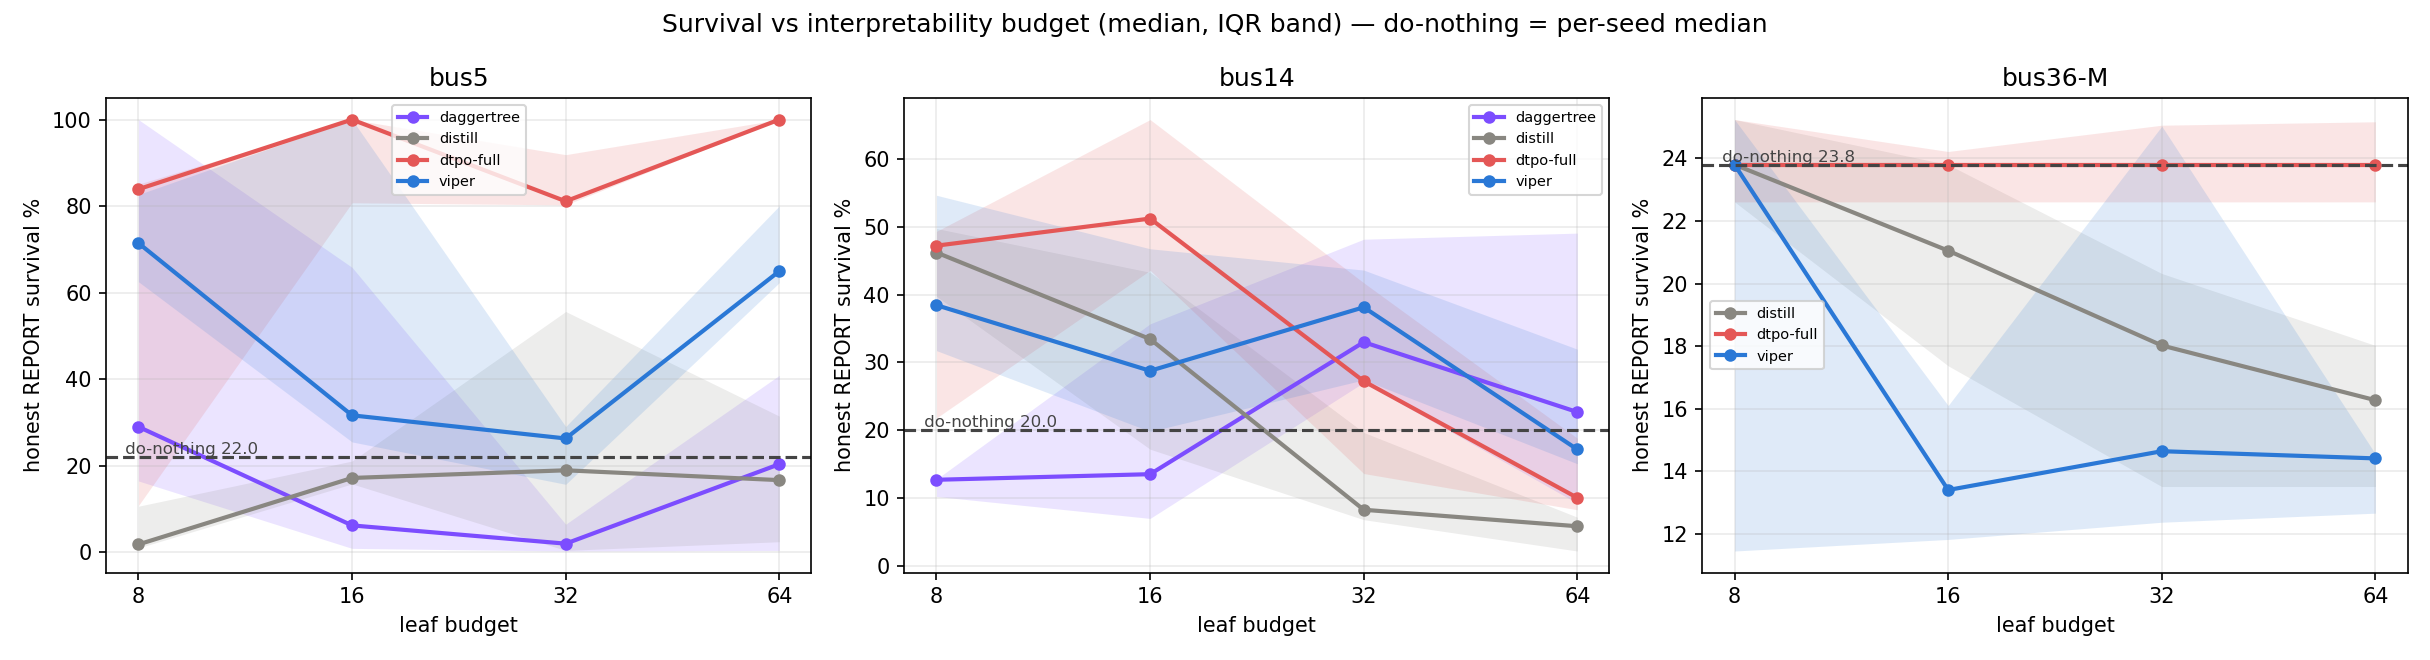
\includegraphics[width=\textwidth]{figures/frontier.png}
\caption{Median report survival against leaf budget, per method and grid, with
the interquartile band. The trade-off inverts on bus14: 8--16 leaves dominates
64.}
\label{fig:frontier}
\end{figure}

A plausible explanation as to why GDTPO performs better at 16 leaves, whereas VIPER and DAgger perform better with more leaves is that more leaves provides methods like VIPER and DAgger a greater breadth to reproduce the actions of the teacher. On the other hand, policies like GDTPO and one-shot distillation differ by actively optimising within the environment itself, instead of fully relying on the teacher oracle (albeit they do utilise it for initial policy establishment). Regardless, one thing that can be corroborated once again is the importance of seed selection as well as the requirement for more tests to obtain more data for quality assurance and ensuring consistency.

\begin{figure}[H]
\centering
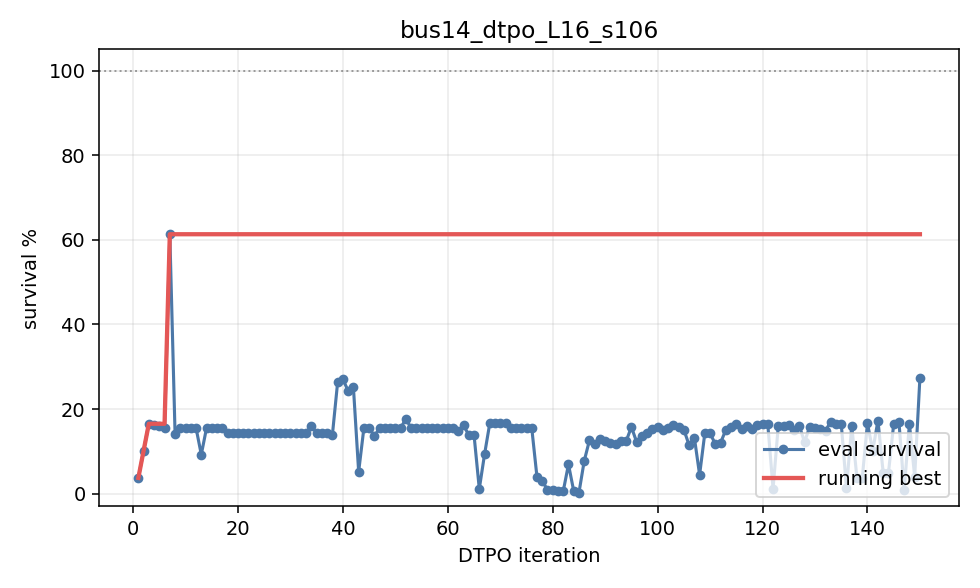
\includegraphics[width=0.85\textwidth]{figures/dtpo_l16_s106.png}
\caption{A single training run (\texttt{bus14\_dtpo\_L16\_s106}):
per-evaluation deployed survival and running best across the 150 iterations.}
\label{fig:curve}
\end{figure}

\begin{figure}[H]
\centering
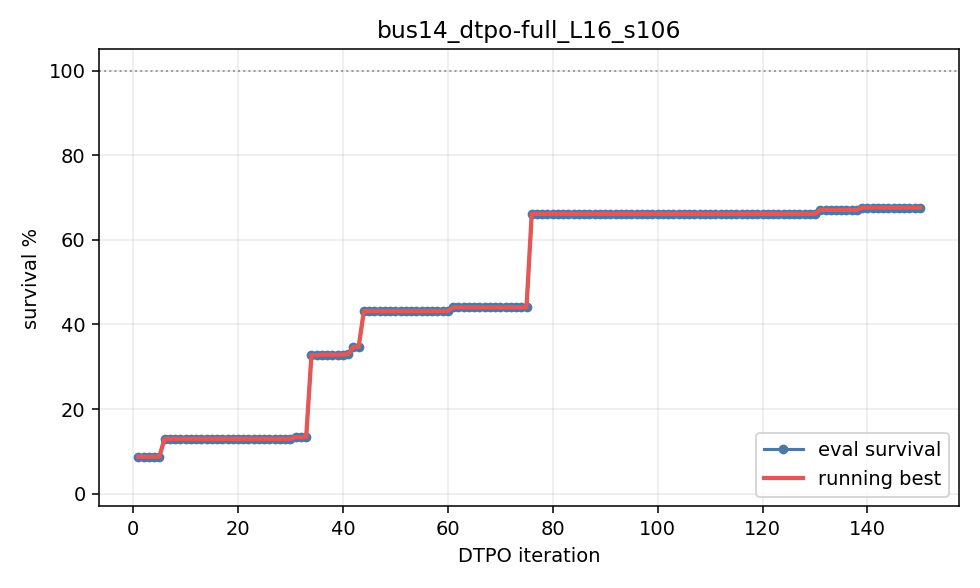
\includegraphics[width=0.85\textwidth]{figures/curve_dtpo-full_s106.png}
\caption{A single training run (\texttt{bus14\_dtpo-full\_L16\_s106}):
per-evaluation deployed survival and running best across the 150 iterations.}
\label{fig:curve2}
\end{figure}

Without the presence of a survival gate, training is erratic and unstable, especially when interpretable policies are being developed. This is seen within black-box models as well, with small improvements as the number of training timesteps and iterations increases, but this is extremely time-consuming and resource-demanding. The inclusion of a survival gate does not necessarily help improve the policy, but rather ensures that a new policy is always at least better than or equal to the previous policy it replaces, and therefore serves as a positive addition to the model for this domain.

% This is showcased in \ref{fig:gate-filter}. 

Although all results report the survival rate, as it is the primary metric that we have based our evaluation on, it should be noted that the cost of evaluation of every policy is considerable. For all policies except one-shot distillation from the PPO oracle, each policy is run for 150 iterations, each including 10,000 timesteps. This gives a combined total of 1.5 million timesteps. On the other hand, the one-shot distillation policy only runs for 20,000 environmental timesteps, with no active reinforcement learning taking place. 

\section{Policy Visualisation}

\begin{figure}[H]
\centering
\includesvg[width=\textwidth,inkscapelatex=false]{figures/tree_warmstarted_s106}
\caption{A warm-started 16-leaf policy on bus14
(\texttt{dtpo-full}, seed 106).}
\label{fig:tree-warm}
\end{figure}

\begin{figure}[H]
\centering
\includesvg[width=\textwidth,inkscapelatex=false]{figures/tree_fromscratch_s100}
\caption{The same budget trained from scratch
(\texttt{dtpo-scratchfull}, seed 100), for comparison with
Figure~\ref{fig:tree-warm}.}
\label{fig:tree-scratch}
\end{figure}

% \begin{figure}[H]
% \centering
% 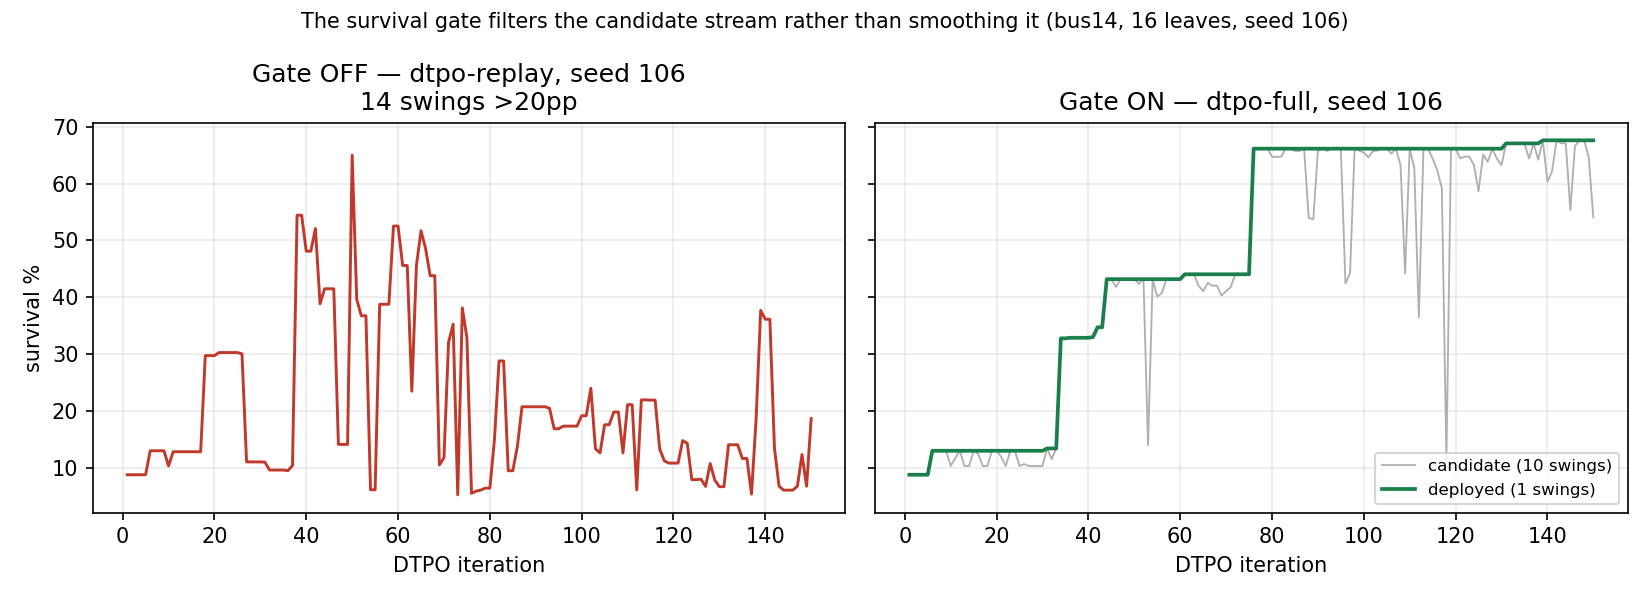
\includegraphics[width=\textwidth]{figures/gate_before_after_s106.png}
% \caption{The survival gate as a filter (bus14, 16 leaves, seed
% 106).}
% \label{fig:gate-filter}
% \end{figure}


Within the visualisation of the trees, each node consists of the observation attribute and a comparative with a value, and its leaves consist of two variables, namely the action as well as its respective $p$, the average probability assigned to this action by the stochastic policy. As the tree is fit as a regressor onto a normalised target over distributed actions, the action with the largest $p$ is finally chosen. Although the policy during training is stochastic, the deployed policy through the interpretable decision tree is ultimately deterministic. The closer the value of $p$ is to 1.00, the more likely the policy preferred this action, and vice versa; the closer the value of $p$ is to 0.02 (since there are 50 actions possible in total, making 0.02 the uniform value), the more equally probable each possible action was. 

This does not fully indicate that some trees are more confident than others. Within the strongest interpretable policies trained, we see that some leaves showcase $p$ up to 0.99, showcasing high confidence, whereas other leaves may have a $p$ as low as 0.04. By this understanding, the results of bus36-M may be construed to be anomalous, since some seeds contain nodes with both child leaves showcasing the action 0 of ``do-nothing'' with $p = 1.00$, essentially reverting to exactly the same policy as do-nothing. This could be due to two reasons. The first is that the policies truly converge towards the do-nothing action, as the teacher policy itself tends to idle and rarely produces other actions that have an impact on the environment. But since the policies of DTPO configurations trained from scratch tend to return the exact same values as that of the do-nothing policies, this suggests a discrepancy between the actions suggested by the decision tree from its policy learning, and the action space itself. We observe that some seeds within bus36-M, such as seeds 101 and 103, do showcase other actions in their leaves, yet still output the same policy as do-nothing. These actions specifically are actions that allow for more than one substation to be changed within the same timestep. Thus, this suggests that the environment is unable to accept actions that impact more than one substation simultaneously, causing a revert to the default do-nothing action. This is another reason why the bus36-M results are not prioritised, and bus14 and bus5 are preferred in that order, as the anomalous data of bus36-M can be attributed to the inherent action space file being inconsistent with the environment itself. This will require further testing to confirm this hypothesis, and shall be detailed in future work. 

The value of $p$ has been intentionally included such that human-operators utilising these decision trees to take decisions will be able to understand how confident the policy is in choosing a certain action for a leaf. 

\section{Fidelity}

Through fidelity, we aim to measure whether a distilled policy is able to reproduce the actions of its teacher oracle. Each policy is measured on two state distributions: those visited by the oracle, and those visited by the tree itself. Both use the same environment, evaluation, and start, only differing in the action executed, thereby showcasing the divergence in trajectories. The former questions whether the tree is able to learn how the teacher operates in its trajectory, whereas the latter questions whether the actions suggested agree even when the trajectory of the environment changes due to the actions of the tree. Measurements are done over ten episodes per run, and shown in Table~\ref{tab:fidelity}. We observe that every configuration loses fidelity moving from the oracle-visited states to the tree-visited states. This loss is unsurprisingly smallest for the imitation methods like one-shot distillation (\textit{distill}) and DAgger, where the average weighted fidelity falls from 0.799 to 0.620 and 0.746 to 0.527 respectively.

\begin{table}[H]
\centering
\footnotesize
\setlength{\tabcolsep}{4pt}
\begin{tabular}{lrrrrrrrrr}
\toprule
& & \multicolumn{4}{c}{on oracle-visited states} & \multicolumn{4}{c}{on tree-visited states} \\
\cmidrule(lr){3-6}\cmidrule(lr){7-10}
& & \multicolumn{2}{c}{fidelity} & \multicolumn{2}{c}{weighted} &
    \multicolumn{2}{c}{fidelity} & \multicolumn{2}{c}{weighted} \\
\cmidrule(lr){3-4}\cmidrule(lr){5-6}\cmidrule(lr){7-8}\cmidrule(lr){9-10}
method & $n$ & med & mean & med & mean & med & mean & med & mean \\
\midrule
\texttt{distill} & 10 & 0.606 & 0.612 & 0.801 & 0.799 & 0.497 & 0.483 & 0.659 & 0.620 \\
\texttt{daggertree} & 10 & 0.557 & 0.556 & 0.747 & 0.746 & 0.470 & 0.398 & 0.648 & 0.527 \\
\texttt{viper} & 10 & 0.437 & 0.442 & 0.589 & 0.564 & 0.382 & 0.371 & 0.494 & 0.481 \\
\texttt{dtpo-gate-K1} & 10 & 0.441 & 0.445 & 0.506 & 0.500 & 0.134 & 0.153 & 0.200 & 0.180 \\
\texttt{dtpo-gate} & 10 & 0.432 & 0.435 & 0.502 & 0.512 & 0.163 & 0.199 & 0.238 & 0.247 \\
\texttt{dtpo-full} \emph{(GDTPO)} & 10 & 0.420 & 0.415 & 0.501 & 0.496 & 0.213 & 0.219 & 0.245 & 0.261 \\
\texttt{dtpo-ws} & 10 & 0.385 & 0.395 & 0.412 & 0.452 & 0.177 & 0.182 & 0.180 & 0.196 \\
\texttt{dtpo-replay} & 10 & 0.381 & 0.370 & 0.390 & 0.393 & 0.184 & 0.180 & 0.234 & 0.217 \\
\midrule
\texttt{dtpo-scratchfull}$^{\dagger}$ & 10 & 0.207 & 0.182 & 0.117 & 0.110 & 0.002 & 0.018 & 0.001 & 0.012 \\
\texttt{dtpo-scratchgate}$^{\dagger}$ & 10 & 0.134 & 0.136 & 0.101 & 0.116 & 0.042 & 0.104 & 0.032 & 0.137 \\
\texttt{dtpo}$^{\dagger}$ & 10 & 0.063 & 0.103 & 0.038 & 0.059 & 0.007 & 0.028 & 0.009 & 0.030 \\
\bottomrule
\end{tabular}
\caption[Tree--oracle fidelity on bus14]{%
\textbf{Fidelity between each distilled tree and the PPO teacher} on bus14 at a
sixteen-leaf budget, over ten seeds. Rows are ordered by weighted fidelity on oracle-visited states. Configurations marked $\dagger$ were trained without a teacher.}
\label{tab:fidelity}
\end{table}

As we are aiming to optimise the survival rate, the inclusion of a teacher oracle via the warm start mechanism does improve the fidelity, but invariably do not reach the same fidelity as the pure imitation methods. As anticipated, the three counterparts which were trained without a teacher showcase the lowest fidelity, with the original DTPO method possessing a mean weighted fidelity of 0.059. This confirms that the presence of the teacher oracle during training does have an impact on the similarity of the policies between the teacher and the student.

Compared against the survival rate results in Table~\ref{tab:headline}, we see there is no clear indication that fidelity and survival rate go hand in hand. Configurations like \texttt{dtpo-scratchgate} have one of the lowest fidelity rates, as it was not trained with the teacher oracle, but attains an average survival rate higher than one-shot distillation, which attained the highest fidelity values across the eleven configurations on bus14. 

A limitation of this fidelity study is that we only compare the behaviour of our configurations on a specific PPO oracle teacher checkpoint. Furthermore, survival and fidelity are heavily dependent on the trajectory of the environment based on the actions taken; since the fidelity is calculated as a ratio measuring the similarity between the actions of the teacher and the student, the fidelity value can immediately derail, depending on how earlier a discrepancy occurs between the two. 

\section{Discussion}


Several aspects of this research were found to be difficult to navigate, and all factors will be discussed here in detail as the project's limitations and threats to validity.

\textbf{Seed selection.} Since each seed of the environment selects its own set of chronics, where each series of chronics differs in difficulty, it is extremely challenging to produce reliable and stable checkpoints across all seeds. This was the reason why the chronics evaluated upon were fixed; even though the consistency and stability can be improved through a greater number of tests, the CPU resources required would be extensive, which is why our runs were limited to a maximum of ten per method tested.

\textbf{Chronics.} Additionally, our choice of chronics may have also swayed the selection and choice of the decision trees. Due to both resource and time constraints, all the remaining chronics were not used for validation and testing, and this could be changed within the methodology for a better understanding of how the decision trees would perform in more environment scenarios.

\textbf{Teacher oracle.} Checkpoints trained by the benchmark do not store the observation normalisation statistics under which the policies are trained, and so it is difficult to evaluate or reproduce the policy unless the environment and agent seed are known. To ensure stability of the teacher oracle, we therefore obtained the final checkpoints of the PPO teacher oracle of bus5 and bus14 directly from the authors of RL2Grid, which saved significant training time. The training of the bus36-M oracle took over three continuous weeks on a local machine. Initial testing within the interim report also focused on identifying strong DQN oracles, but these were disregarded due to their instability and weakness in comparison with their PPO counterparts. Therefore, further testing is required to test the methods and complete an ablation study on multiple teacher oracles, rather than only one. Methods like VIPER are also primarily designed to distil a complex deep neural network policy, making DQN oracles the better choice. However, due to the availability and strength of PPO oracles, the implementation of VIPER was therefore adapted to not only fit the requirements of RL2Grid, but also obtain the action-probability gap between the top two actions as a replacement for the lack of Q-values in the stochastic policy.

\textbf{Training cost.} The cost of training and evaluation played a crucial role in the design of these experiments. Given the computational resources, the number of iterations can also be increased further, to see the impact on training and testing and observe at which point the survival rate saturates and plateaus in its growth. Given the size and complexity of the environment, and time taken for training any policy, the number of iterations had to be limited to 150. It remains completely possible that the published algorithms as well as our improved algorithm showcase improvement on all grid types as the opportunity for compute increases. Furthermore, solely looking at the results elaborated upon within this Chapter totals approximately 2,500 hours of CPU wall time, which excludes the plethora of CPU hours spent on countless other sweeps during testing across the duration of the project. The bus14 PPO teacher oracle was trained on 45 million environment steps. This cost has significantly limited our intention to test on multiple seeds and ot test methods more than 10 times, and this remains to be further delved into.

\textbf{Fickle fidelity.} The imitation-based policies aim to maximise fidelity, trying to ensure that the student policy agrees with the teacher oracle as much as possible. Our method, where the oracle is used as the foundation for its own policy (prior to further refinement) also initially follows this path, before optimising on its own. Nevertheless, higher-fidelity decision trees do not necessarily have high survival rates, and vice-versa; the policies with the highest survival rate tend to deviate from the teacher oracle. Within this study, no single configuration jointly maximised survival rate and fidelity. We hypothesise that within power grid operations, there is no true optimal policy in successfully handling a complete grid environment, as its complexity (especially as the grid size increases) makes it extremely challenging to have a singular policy that is able to solve the environment. Additionally, the variation of the trajectory through the environment itself can allow multiple policies to attain the same survival rate while differing in actions taken.


\textbf{Ethical and societal considerations.} \label{sec:discussion} It should be duly noted that although our proposed method is able to definitely beat the original algorithm within this specific domain based on our experimentation, this is not a policy that should be given control of any power grid network. More importantly, the same could be said about any of the black-box oracles themselves, as they struggle to generalise and learn policies that have strong survival rates as the complexity of the environments increases. Nonetheless, although these policies should not be deployed, they are an excellent step towards providing support to human operators in their decision-making process. Simply because we have included the property of interpretability within our interpretable policies, it does not mean that reliability has inherently made itself a part of the policies as well, and requires much further evaluation utilising more metrics for a complete guarantee of the findings. 

\section{Reflection}

\textbf{Deviation from interim results.} Preliminary experiments also tested other neuro-symbolic methods such as S-REINFORCE, but these policies showcased the weakest performance. This could be due to the complexity of the action space, and the symbolic regressor being unable to mathematically approximate the neural network's policy. Moreover, initial plans considered techniques such as pruning and hyperparameter tuning to identify improvements to survival rate performance, but these were not prioritised in favour of a consistent evaluation framework and the ablation study of GDTPO. Further fine-tuning via a hyperparameter configuration grid search may undoubtedly work towards improvement within this domain.  

\textbf{Novel contribution was successful, but scalability was not.} To the best of our knowledge, the approach of implementing GDTPO and DTPO within the context of power grids has not been implemented before. Alongside a consistent replicable evaluation framework, we have achieved the goals sought after. However, it was initially planned to obtain results for bus118-M as well, but that grid did not yield a usable teacher oracle for either PPO or DQN, and was therefore not considered. The fallback of bus36-M policies onto the do-nothing policy also indicates that further debugging is required on its action space.  

\textbf{Multi-agent interpretable policies require significant work.} Approximately one month of this project was devoted towards a faithful implementation of MAVIPER \cite{milani2022maviper} within the multi-agent topology task. Despite this, we were limited by the strength of the teacher oracle policy itself to obtain useful data, as these teacher policies were undertrained and required significant CPU wall time that was unavailable given our project timeline. Once again, we highlight the importance of the teacher oracle, even if it is a black-box model, in order to work towards training valuable interpretable models.

\chapter{Lessons Learned}
\label{ch:lessonslearned}

In this chapter, we aim to accumulate all the lessons we have learned throughout this project. By focusing on the challenges that come with the technical problem of explainable reinforcement learning within power grid systems, we aim to highlight the key takeaways that one must grasp prior to conducting further research in this field. 

\section{Scalability and Complexity}

Current grid operators continue to modify substations and transmission lines manually, taking into consideration the behavioural history of the grids themselves. At the time of writing, there exists no optimal solution that can completely solve a grid system and still scale without degradation of performance and robustness. Therefore, it is vital that we continue to explore this direction, as scalability continues to be the core issue to improve the realism of policies. Many of the existing simulation environments, such as Grid2Op and RL2Grid, are built upon synthetic data. Work must be done to publicly and safely release grid data that is representative of true grid environments, without infringing upon the privacy of transmission companies and being mindful of international policies with regards to power grid systems. Thus, scalability and complexity remain to be critical challenges within power systems.

\section{Idleness Can Dominate on Low Difficulty}

% Based on current baselines on easy difficulty, doing nothing can be competitive

Within smaller grids, such as the three tested within this project, denying the agent control of the environment and allowing the environment to continue without any external intervention seems to improve the performance of trained policies. This is most visible when the difficulty of the environment is low. This can create a bias for policies to continue performing the idle action to substantially boost their reward. Therefore, more data is required for power grid systems where abnormal changes to the grid are highlighted, such that policies can be truly evaluated for whether they showcase strong performance. Additionally, the inclusion of external sources such as VREs and batteries will continue to increase uncertainty and instability within grid networks. Even grids like bus36-M are extremely simple relative to national and global transmission systems, and are not truly reflective of the complexity that these grids can reach.

\section{Time Constraints}

% 

% gpu accelerated environment simulation, parallelise thousands of grid environments simultaneously, use libraries like JAX, computationally heavy

Environment simulations will continue to take time as long as they stay CPU-bound. It takes thousands of CPU wall time hours to explore this field of work and conduct meaningful experiments, just to push the envelope of current benchmarks. This is extremely computationally heavy, let alone time-consuming. Although RL methods rely on the CPU for environmental simulations due to their sequential behaviour, research will continue to take significant time if we stick to this precedent, especially given the complexity of power grid systems. To tackle this predicament, research must be conducted to incorporate GPU-accelerated environment simulation within existing benchmarks, such that training can parallelise hundreds and thousands of grid environments simultaneously. Libraries like JAX can be taken advantage of for bringing this into fruition.

\section{Limited Intrinsic Research}

% Intrinsic methods are extremely understudied

Due to the issue of scalability, the entire domain of ante-hoc methods continues to stay within uncharted territory, understudied and neglected in favour of more blooming topics within RL, such as post-hoc methods and counterfactuals. Current work does delve into neuro-symbolic models, but intrinsically interpretable models that are both small and sparse remain an open question. This project delved into this domain to stay ambitious within intrinsically interpretable methods. Counterfactuals were considered as a contingency plan, but a pivot towards frameworks that incorporate it was not made as they typically assume centralised control and have non-cooperative agents, some of which have joint policies. This is more useful when exploring multi-agent RL, which was touched upon but not explored in depth for this project, once again due to computational and time constraints. Counterfactuals do provide structural explanations (such as which agents cooperated, and in what order actions took place), but do not possess causal attributions (such as highlighting which intervention truly mattered towards the performance of the policy). Given issues with overgeneralisation and the lack of a causal model, this too remains an open challenge. 

% focus on post-hoc and counterfactuals

\section{Black-Box Model Strength}

% \section{Teacher Policy}

Regardless of whether one explores post-hoc methods or intrinsically interpretable policies, single-agent or multi-agent, one conclusion that can be taken from this work is that the optimal outcome of student policies being able to match or exceed the performance of teacher oracles themselves is currently far-fetched. The teacher policies themselves have their own limitations, unable to reach strong survival rates as the grid complexity increases. 

It is vital that current reinforcement learning research within power grid operations is focused upon training good black-box models that generalise well, especially when considering scalability and complexity of grids. The largest improvement in interpretable student policies is observed when the teacher oracle policy is strongest, as seen by the generalisation of all policies on bus5, compared to the variation in interpretable policies trained on bus14. Regardless of optimisation techniques, the student policy is unable to exceed the teacher oracle, the latter thereby establishing itself as the current upper bound. 

Thus, the best performance currently will still be determined by black-box models, and we must strive towards improving these methods first, before aiming to explain how and why they work. Popular baselines and techniques like PPO and DQN have continued to revolutionise the reinforcement learning community for the last decade. Yet, the performance of these state-of-the-art methods within power grid systems showcases that there still exists a plethora of room for improvement to attain high, robust performance and survival within these grids. The performance of interpretable policies will ultimately be dictated by teacher quality.

% state-of-the-art, popular baselines, still significant room for improvement in the performance of these methods

%  Furthermore, retraining these teacher oracles was not possible, as training a black-box policy up to 45 million timesteps required over 4 weeks of continuous CPU wall time, which was not feasible given the time constraints of the project. Therefore, significant work is required in this field to further strengthen the teacher policy, before further research is conducted within explainable methods, especially if interpretable techniques are delved into.
\chapter{Conclusion}
\label{ch:Conclusion}

% Conclusion - 2 pages

In this thesis, we set out to investigate whether interpretable reinforcement learning methods can produce controllers that are not only transparent, but also operationally reliable in power grid environments, whilst maintaining high operational metrics. Drawing from existing interpretable methods, we designed a modified and improved algorithm that utilises decision tree policy optimisation, which we have coined as GDTPO. Through this work, we were able to produce intrinsically interpretable policies, yet were also able to identify that this domain holds many open research questions and requires further work in ensuring high operational reliability and stability. Several key findings emerged, which have shaped the lessons learned from this project.

\section{Future Work}

\subsection{Multi-Agent Topology Control}

Current research within power grid operations seems to showcase that single-agent policies have stagnated, with current work tackling whether multi-agent policies can solve this complex domain \cite{marchesini2026marl2grid}. True transmission control is not centralised, with a multitude of grid operators handling portions of the grid, especially when these networks can be as vast as that of a country. A single agent is unable to scale as the size of the grid and the number of substations increases. Thus, there is current work within decentralised agents, each handling their own domain within the grid, in order to tackle the issue of scale.

Even within multi-agent reinforcement learning, there must be substantial research put not only towards training strong teacher policies with stable checkpoints, but studies must be conducted in order to work towards global interpretability, instead of solely focusing on local interpretability of each agent on the grid. This research direction of working on local-to-global interpretability is the most prominent question that remains unanswered within this field of explainable multi-agent reinforcement learning within power grid operations.

\subsection{Generalisation}

Although we are confident of our improved algorithm's behaviour and performance, these improvements are still domain-specific. Additionally, the original DTPO algorithm was tested within typical reinforcement learning domains such as CartPole, where training policies is much less resource-demanding. To confirm the generalisation of our GDTPO algorithm across all domains of reinforcement learning, testing must be conducted within these domains, certifying it as a valid contribution to the reinforcement learning space.

Due to the complexity of the research question and the environment itself, the work was intentionally limited to the lowest difficulty with a maximum of 50 actions, and our domain was limited to topological control. Theoretically, it is possible to explore redispatch control, where continuous actions are also possible. If the direction of developing decision trees is taken within redispatch, then the concept of discretising the action space must be explored.

Moreover, resources used by current reinforcement learning methods within power grid operations seem to be strictly limited to CPU usage. Foregoing the use of GPUs for training and testing significantly impacts the progress of research and evaluation, and this is a vital aspect that must be tackled in order to vastly speed up and develop improvements within this field.

\subsection{Post-Hoc Interpretability}

Our work intentionally delved into interpretable models, instead of going in the more extensively researched direction of post-hoc methods such as feature importance or development of concept-based explainability frameworks. Post-hoc explainable policies are not intrinsically interpretable, but due to the current limitation of scalability within decision trees, especially as the number of actions and the grid size increases, both may be used alongside one another to complement each other. This remains an open challenge within the research community that requires further study. 

Further studies can also be conducted using a human-in-the-loop approach to evaluate the methods against one another, as well as benchmark against subject matter experts and operators who have substantial experience in their domain. For this work, proxies like fidelity and number of leaves of the decision tree were used for evaluation purposes. Future work can observe application-based evaluation, which includes a human expert working within a real environment for comparison against the interpretable model.

\section{Final Contributions}

Through this work, we successfully gained a thorough insight into reinforcement learning strategies within power grid operations, understanding the various techniques within intrinsically interpretable models, as well as the trade-offs being balanced between attaining a high survival rate while ensuring transparency and interpretability of the policy. 
We were able to confirm that current state-of-the-art methods for training interpretable reinforcement learning policies are able to inadequately preserve operational performance in power grid topology environments, limited in their survival performance to an upper bound of their black-box teacher oracle policies.

Through the implementation of existing approaches like VIPER and DAgger, we have mapped the landscape of what is possible for intrinsically interpretable methods within explainable reinforcement learning methods for power grid operation. Through this work, we proposed GDTPO, a novel approach that builds upon and improves existing interpretable policy extraction methods through four major modifications. GDTPO is able to recover on average 77.8\% of its PPO black-box teacher within a 16-leaf tree on the bus14 environment, indicating that GDTPO is a simple yet effective approach. GDTPO's promising results highlight the importance of future research into scalable frameworks that are intrinsically interpretable.

Future work within this domain seems to be vastly open-ended, with the struggles of scalability and generalisation of policies being observed, tied in part to the complexity of not only building intrinsically interpretable models, but also the complexity of the grid environments themselves. Nonetheless, we face an optimistic future within this domain. As power grid operations are extremely high-stakes, it is vital that we continue to understand the reasoning behind the decision-making process of a reinforcement learning model, rather than solely being critical of the action and its performance. It is vital that as researchers, we continue to ask the question of ``why?'' - and this must be raised and answered not only in the work that we do, but also answered by the autonomous models that we build to help shape our society. We look forward to seeing how these methods are improved upon, and are excited about the future work on novel online RL algorithms, that can both influence and speed up the work within power grids as well.





%% bibliography
\bibliographystyle{vancouver}
\bibliography{references}

\chapter{Declarations}
\label{ch:Declarations}

\section{Use of Generative AI}

I acknowledge the use of Claude Code (Anthropic, \url{https://claude.ai/code}) as an assistive tool for programming, such as the debugging of code and scripts, and the extraction and visualisation of metrics from raw logs. Its assistance was also used for manuscript editing, such as the LaTeX formatting of tables and figures. All research designs are solely the original intellectual work of the author, and no (semantic) content generated by Large Language Models (LLMs) has been presented as the author's own work.

\section{Ethical Considerations}

Ethics approval was not required for this project, as all experimentation was conducted on simulated frameworks of power grid systems. Ethical and societal considerations are discussed within Section~\ref{sec:discussion}.

\section{Sustainability}

Although experimentation and testing were computationally heavy, all model training and environment simulations were limited to shared CPU infrastructure. Significant training and experimentation were also avoided by the use of saved checkpoints, especially with regard to the reuse of the teacher oracle, which substantially reduced computation. 

\section{Availability of Data and Materials}

The source code for the Grid2Op platform that allows for power grid control can be found publicly at \url{https://github.com/Grid2op/grid2op}. The original source code for the RL2Grid benchmark can be found at \url{https://github.com/emarche/RL2Grid}. The code developed for this project, which builds upon the RL2Grid benchmark, and includes all training and testing outputs, can be found at \url{https://github.com/saisurag/IRL2Grid}. The checkpoints of the methods trained and tested can be found at \url{https://github.com/saisurag/IRL2Grid-checkpoints}, and can also be downloaded as a .zip file at the Google Drive link below. A separate repository has been created specifically for the checkpoints in consideration of storage. \url{https://drive.google.com/file/d/1Pb0b8U6JRertQdG9igteh-RTTkOoG417/view?usp=drive_link}.

\end{document}